%\PassOptionsToPackage{english}{babel}

\documentclass[
	openany,
	% -- opções da classe memoir --
	12pt,				% tamanho da fonte
   % openright,
	%twoside,
    oneside,
    % para impressão em verso e anverso. Oposto a oneside
	a4paper,			% tamanho do papel. 
	english,
	brazil				% o último idioma é o principal do documento
	]{abntex2}

% ---
% Pacotes básicos 
% ---


%\usepackage{helvet}
%\renewcommand{\familydefault}{\sfdefault}

%\usepackage{fontspec}
%\setmainfont{Arial}

\usepackage{lmodern}			% Usa a fonte Latin Modern			
\usepackage[T1]{fontenc}		% Selecao de codigos de fonte.


\usepackage[utf8]{inputenc}		% Codificacao do documento (conversão automática dos acentos)
\usepackage{indentfirst}		% Indenta o primeiro parágrafo de cada seção.
\usepackage{color}				% Controle das cores
\usepackage{graphicx}			% Inclusão de gráficos
\usepackage{microtype} 			% para melhorias de justificação
\usepackage{multicol}			% multiplas colunas no texto
\usepackage{multirow}
\usepackage{subcaption}
\usepackage{caption}
\usepackage{float}
\usepackage{amsmath}
\usepackage{amssymb}
\usepackage{amsthm}
\usepackage{lipsum}
\usepackage{amsmath}
\usepackage{blindtext}
\usepackage{csvsimple}

\usepackage{tabularx}
%\usepackage{url}
%\usepackage{hyperref}


% ---
% ---
% Pacotes de citações
% ---
\usepackage[brazilian,hyperpageref]{backref}	 % Paginas com as citações na bibl
\usepackage[num]{abntex2cite}	% Citações padrão ABNT

\usepackage{pdfpages}

% --- 
% CONFIGURAÇÕES DE PACOTES
% --- 

\renewcommand{\arraystretch}{1.2}

% ---
% Configurações do pacote backref
% Usado sem a opção hyperpageref de backref
\renewcommand{\backrefpagesname}{Citado na(s) página(s):~}
% Texto padrão antes do número das páginas
\renewcommand{\backref}{}
% Define os textos da citação
\renewcommand*{\backrefalt}[4]{
	\ifcase #1 %
		Nenhuma citação no texto.%
	\or
		Citado na página #2.%
	\else
		Citado #1 vezes nas páginas #2.%
	\fi}%
% ---


\DeclareMathOperator*{\argmin}{arg\,min}
\DeclareMathOperator*{\argmax}{arg\,max}

% ---
% Informações de dados para CAPA e FOLHA DE ROSTO
% ---
\titulo{Aprendizado profundo com capacidade computacional reduzida: uma aplicação à quebra de CAPTCHAs.}
\autor{Diogo Felipe Félix de Melo}
\local{Recife}
\data{Julho de 2018}
\orientador{Pablo de Azevedo Sampaio}



\instituicao{%
	Universidade Federal Rural de Pernambuco -- UFRPE
  	\par
  	Departamento de Computação
    \par
	Bacharelado em Ciências da Camputação
}

\tipotrabalho{Trabalho de Conclusão de Curso}
% O preambulo deve conter o tipo do trabalho, o objetivo, 
% o nome da instituição e a área de concentração 
\preambulo{Monografia apresentada ao Curso de Bacharelado em Ciências da Camputação da Universidade Federal Rural de Pernambuco, como requisito parcial para obtenção do título de Bacharel em Ciências da Camputação.}
% ---


% ---
% Configurações de aparência do PDF final

% alterando o aspecto da cor azul
\definecolor{blue}{RGB}{41,5,195}

% informações do PDF
\makeatletter
\hypersetup{
     	%pagebackref=true,
		pdftitle={\@title}, 
		pdfauthor={\@author},
    	pdfsubject={\imprimirpreambulo},
	    pdfcreator={LaTeX with abnTeX2},
		colorlinks=true,       		% false: boxed links; true: colored links
    	linkcolor=blue,          	% color of internal links
    	citecolor=blue,        		% color of links to bibliography
    	filecolor=magenta,      		% color of file links
		urlcolor=blue,
		bookmarksdepth=4
}
\makeatother
% --- 

% --- 
% Espaçamentos entre linhas e parágrafos 
% --- 

% O tamanho do parágrafo é dado por:
\setlength{\parindent}{1.3cm}

% Controle do espaçamento entre um parágrafo e outro:
\setlength{\parskip}{0.2cm}  % tente também \onelineskip

% ---
% compila o indice
% ---
\makeindex
% ---

% ----
% Início do documento
% ----
\begin{document}

% Seleciona o idioma do documento (conforme pacotes do babel)
%\selectlanguage{english}
\selectlanguage{brazil}

% Retira espaço extra obsoleto entre as frases.
\frenchspacing 

% ----------------------------------------------------------
% ELEMENTOS PRÉ-TEXTUAIS
% ----------------------------------------------------------
% \pretextual
%\begin{figure}[h]
%\centering % este comando é usado para centralizar a figura
%
\includegraphics[width=7cm]{figuras/logo_ufrpe_horizontal.png}\\
%\end{figure}

% \begin{figure}[ht]
% \centering
% \begin{minipage}[b]{0.45\textwidth}
% 
\includegraphics[height=3cm]{figuras/logo_ufrpe_horizontal.png}
% \end{minipage}
% \qquad
% \begin{minipage}[b]{0.45\textwidth}
% 
\includegraphics[height=2.5cm]{figuras/logo_bsi.pdf}
% \end{minipage}
% \end{figure}

%\begin{minipage}[t]{1\textwidth}
	\begin{figure}[ht]
		
\includegraphics[height=3cm]{figuras/logo_ufrpe_horizontal.png}
		\hspace{5.5cm}
    	
\includegraphics[height=3cm]{figuras/bcc_logo.png}
	\end{figure}    
%\end{minipage}

% ---
% Capa
% ---
\imprimircapa
% ---
% ---
% Folha de rosto
% (o * indica que haverá a ficha bibliográfica)
% ---
\imprimirfolhaderosto
% ---

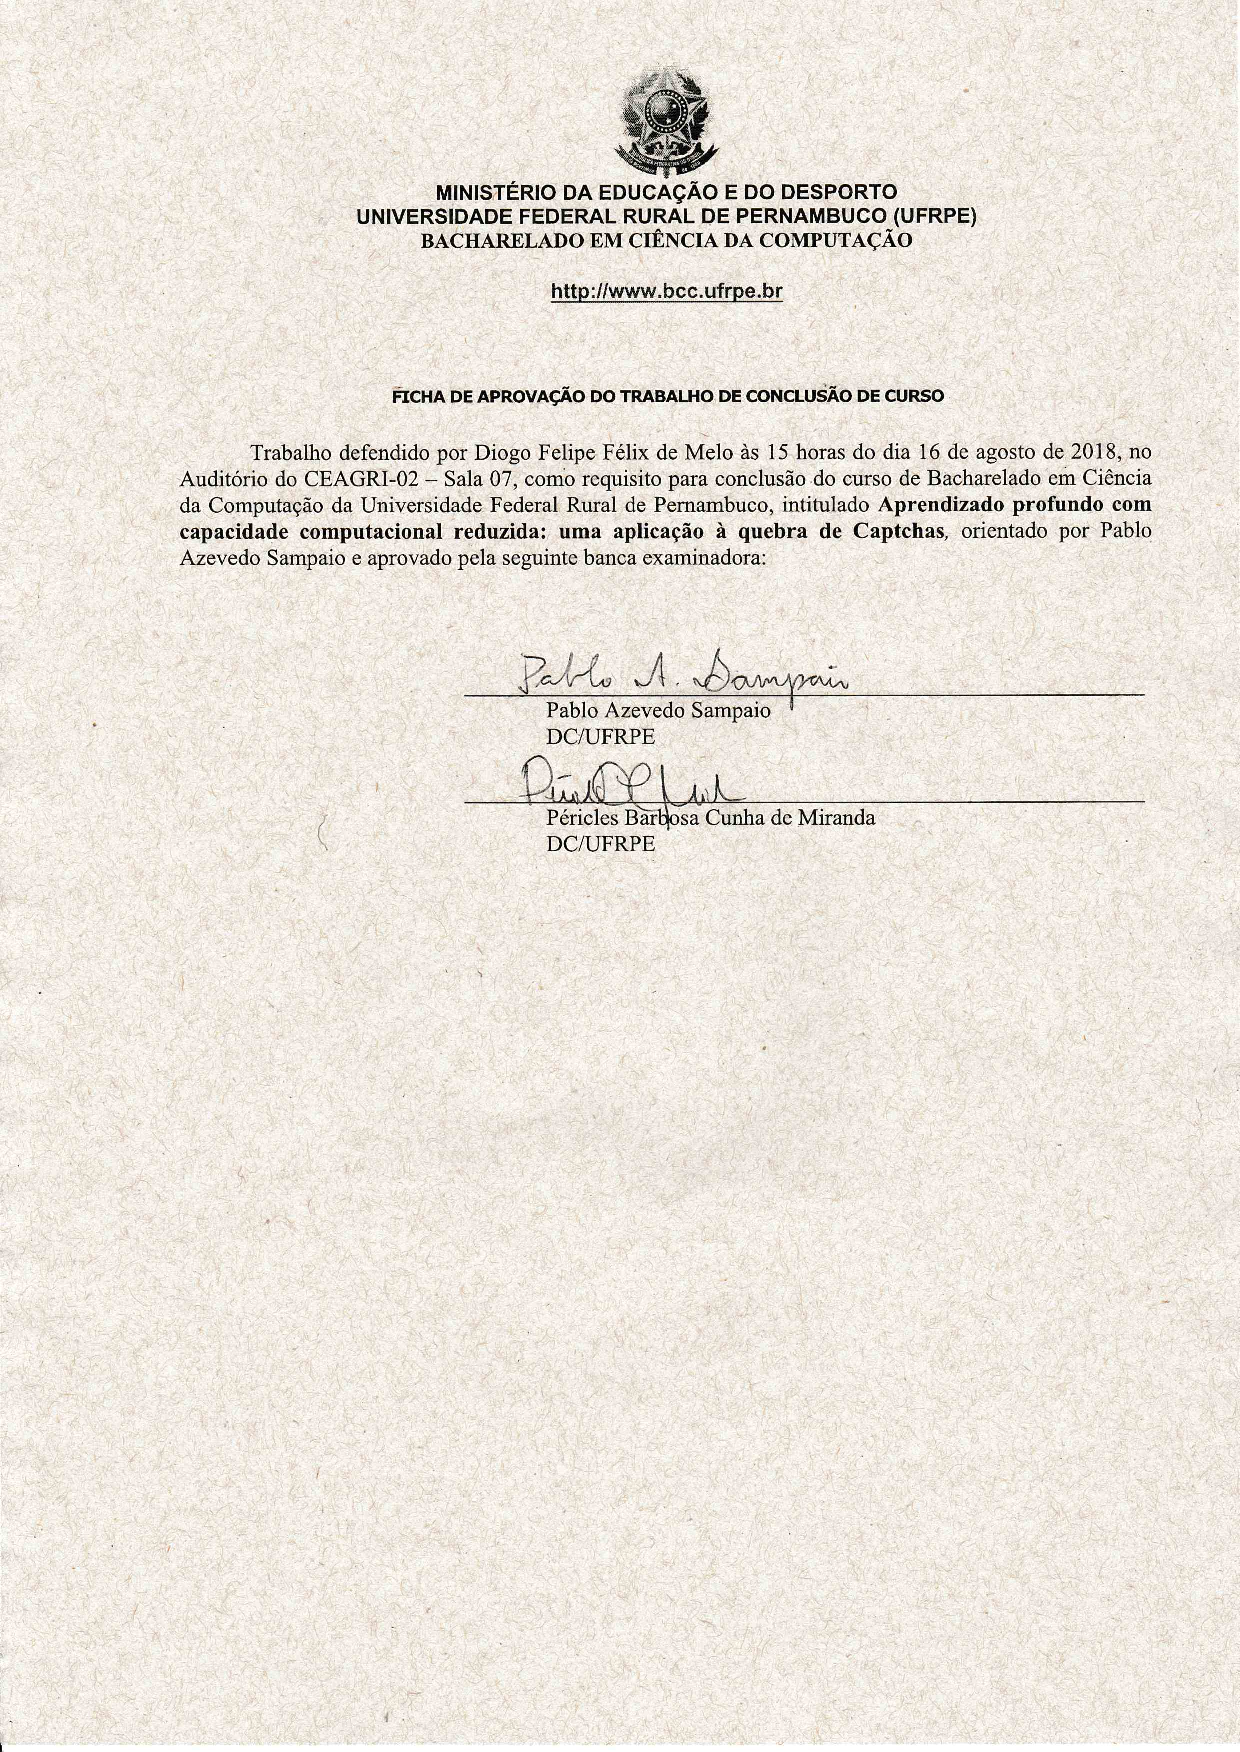
\includepdf[pages={1}]{folhaAprovacao.pdf}

% dedicatoria
%\begin{dedicatoria}
   \vspace*{\fill}
   \centering
   \noindent
   \textit{À \ldots\\} \vspace*{\fill}
\end{dedicatoria}

% agradecimentos
\begin{agradecimentos}

Meus pais, familiares e amigos.

Ao meu orientador, por toda a paciência e dedicação. 

\end{agradecimentos}

% epigrafe
%\begin{epigrafe}
    \vspace*{\fill}
	\begin{flushright}
		\textit{``A persistência é o caminho do êxito.'' \\
		(Charles Chaplin)}
	\end{flushright}
\end{epigrafe}

% resumo e abstract
\setlength{\absparsep}{18pt} % ajusta o espaçamento dos parágrafos do resumo
\begin{resumo}
 



 \textbf{Palavras-chave}: Aprendizado de Maquina, Aprendizado Profundo, CAPTCHA.
\end{resumo}


\begin{resumo}[Abstract]
 \begin{otherlanguage*}{english}
  
During the last decade, Deep Neural Networks has been shown to be a powerfull machine learn technique. Generally, to obtain relevant results, these techniques require high computacional power and large volumes of data. Neverthless, a careful project of trainig and archtecture may help to reduce these requirements. In the this work we present a comparative approach to the application of deep neural networks to text based CAPTCHAs. We studied models that are capable of learn to segment and identify the text content of images, only based on examples. By experimentation of different hiper-parameters and architectures, we were capable to obtain a final model with $96.06\%$ of token prediction accuracy in approximately 3 hours of training in a simple personal computer.
 
   \vspace{\onelineskip}
 
   \noindent
   \textbf{Keywords}: Machine Learning, Deep Learning, CAPTCHA.
 \end{otherlanguage*}
\end{resumo}

% ---
% inserir lista de ilustrações
% ---
\pdfbookmark[0]{\listfigurename}{lof}
\listoffigures
\cleardoublepage
% ---

% ---
% inserir lista de tabelas
% ---
\pdfbookmark[0]{\listtablename}{lot}
\listoftables*
\cleardoublepage
% ---

% ---
% inserir lista de abreviaturas e siglas
% ---
\begin{siglas}
  \item[CAPTCHA] Completely
Automated  Public  Turing  tests  to  tell Computers  and
Humans ApartUser Datagram Protocol
  \item[OCR] Optical Character Recognition

\end{siglas}
% ---

\begin{simbolos}

  \item[$i$, $j$, $k$, $\ldots$] Índices.

  \item[$I$, $J$, $K$, $\ldots$] Conjunto de todos os valores dos índices $i$, $j$, $k$, $\ldots$. $\kappa = (I, J, K, \ldots)$ é uma coleção de índices.

  \item[$\mathbf{x}$] Um vetor.
	 
  \item[$x_i$] Coordenada $i$ do vetor $\mathbf{x}$.
   
  \item[$\mathbf{T^{\kappa}}$] Um tensor com índices na coleção $\kappa$. O tamanho da coleção define o ranque do tensor. Sendo ranque $1$ vetores, $2$ matrizes, etc. Quando definido no contexto, omitiremos $\kappa$.
  
  \item[$T_{i, j, k, \ldots}$] O elemento $i, j, k, \ldots$ do tensor $\mathbf{T}$.
  
  \item[$ \{\ldots\} $] Conjunto de todas as possibilidades de um variável. Usualmente um espaço vetorial.

  \item[$ \langle \ldots \rangle_{D} $] Valor esperado de uma variável no conjunto $D$.

  \item[$| D |$] Número de elementos no conjunto $D$.

  \item[$| \mathbf{T} |_p$] Norma $p$ do tensor $\mathbf{T}$. Quando omitido, $p=2$ (norma euclidiana).

  \item[$\nabla_{\mathbf{T}}$] Operador gradiente com respeito ao tensor $\mathbf{T}$. Isto é, as derivadas em cada elemento de $\mathbf{T}$.
    
  \item[$\Re$] Conjunto dos números reais.
  
  \item[$\Re^{\kappa}$] Espaço dos tensores de ranque $\mathbf{T^{\kappa}}$ sob o conjunto dos números reais. Isto é, $T_{i, j, k, \ldots} \in \Re$.
  
  \item[$ \Re^{\kappa} \lceil \!\!\! \lfloor0,1 \rfloor \!\!\! \rceil $] Compacto dos tensores $\mathbf{T^{\kappa}}$ sob o conjunto $[a,b]$, com $a, b \in \Re$. 
  
  \item[$2^D$] Conjunto de todos os subconjuntos de $D$.
  
  \item[$\mathtt{x}$] Variável aleatória.
  
  \item[$P(\mathtt{x}=a)$] Probabilidade do evento $\mathtt{x}=a$ ocorrer. Quando estiver claro no contexto, utilizamos apenas $P(a)$
  

\end{simbolos}


% ---
% inserir o sumario
% ---
\pdfbookmark[0]{\contentsname}{toc}
\tableofcontents*
\cleardoublepage
% ---



% ----------------------------------------------------------
% ELEMENTOS TEXTUAIS
% ----------------------------------------------------------
\textual

% ----------------------------------------------------------
% inclusao das secoes do texto
% ----------------------------------------------------------
\chapter{Introdução}

Algoritmos de aprendizado baseados em neurologia são conhecidos desde meados do século passado \cite{perceptron_58}. Das proposições iniciais até os dias de hoje, essa classe de modelos tem evoluído em complexidade e técnicas de forma contínua,
culminando em um alto poder de expressividade e níveis cada vez mais abstratos de representação (ver \cite{Goodfellow-et-al-2016} ou \cite{jurgenReview2015} para uma breve revisão histórica). Os poucos resultados teóricos disponíveis demonstram que redes neurais possuem um alto poder de generalização, sendo capazes de, sob certas circunstâncias, codificar diversas classes de funções \cite{Barron1993UniversalAB, Andoni2014PolyAprox}. Apesar dos avanços na área, foi apenas recentemente que modelos neurais começaram a redefinir o estado da arte, superando outras classes de algoritmos de aprendizado de máquina \cite{imagenet_2012} e até mesmo alcançando performances sobre-humanas \cite{mnih2015humanlevel}. Á estes modelos propostos mais recentemente é comum a denominação de redes neurais de aprendizado profundo. Tais avanços foram possíveis devido a três fatores chaves: a viabilização de bases de dados cada vez maiores, o aumento do poder computacional e o desenvolvimento de novas arquiteturas e técnicas de treino.

A crescente melhoria de performance dos modelos neurais de aprendizado profundo tem motivado estudos em áreas onde é preciso distinguir computadores e humanos. Dentre essas áreas temos os CAPTCHAs \cite{captcha2003} (do inglês Completely Automated  Public  Turing  tests  to  tell  Computers  and Humans Apart) ou HIPs \cite{lectures2005HIP} (do inglês Human Interaction Proofs), que definem uma coleção de técnicas que tem como objetivo bloquear a ação de agentes autônomos na rede mundial de computadores. Um dos subconjuntos mais conhecidos dessas técnicas talvez seja o de CAPTCHAs baseados em texto \cite{captcha_review_2017}. Nesse tipo de desafio, uma imagem contendo uma sequência de caracteres é exibida e a validação é feita pela comparação entre o texto informado pelo usuário e a resposta correta. Formulado como um problema de aprendizado de máquina, desejamos descobrir de forma automatizada um mapa entre a imagem e o texto codificado. Na versão informada do problema, um ser humano escolhe previamente técnicas de preprocessamento (filtros, segmentação de caracteres, etc.) antes que o aprendizado propriamente dito ocorra. Ajudados por humanos, redes neurais simples e com poucos exemplos conseguem resultados satisfatórios nesse tipo de desafio \cite{lectures2005HIP}. De fato, mesmo técnicas ingênuas como contagem de \textit{pixels} podem obter bons resultados quando o preprocessamento correto é fornecido \cite{naivecaptcha}. Na versão não informada, entretanto, encontrar mapas imagem-texto de forma automatizada é usualmente muito mais desafiador. Em trabalhos recentes, foram relatados modelos baseados em redes neurais capazes de burlar esse tipo de desafio com acurácias de acerto próximos à humana em sequências sorteadas a partir de um repositório \cite{captcha_break_2013} e modelos com alta eficiência de dados \cite{captcha_break_2017}. Para o problema geral de quebrar CAPTCHAs baseados em texto, entretanto, modelos de aprendizado profundo ainda mostram desempenho inferior ao humano. Contudo, pesquisas recentes apontam para avanços claros nos próximos anos \cite{Bursztein2014TheEI}. Em comum, esses modelos possuem a necessidade de \textit{clusters} e/ou sistemas de computação sob demanda para treinamento, com hardware de alto poder de processamento e/ou paralelização, como GPUs e TPUs. Adicionalmente, as bases de treinamento necessárias comumente alcançam alguns terabytes e envolvem grandes operações de aquisição e/ou geração.

Neste trabalho propomos uma abordagem comparativa entre diferentes arquiteturas de redes neurais para a solução de CAPTCHAs baseados em texto sem informação humana, nos restringindo, entretanto, à um ambiente com poder computacional reduzido. Pretendemos mostrar que é possível fazer uso dessas técnicas em um mero computador pessoal (na contramão dos trabalhos usualmente encontrados na literatura) e ainda obter resultados próximos ao estado da arte. Este trabalho se encontra organizado como segue. No capítulo \ref{cap:captchas} apresentamos uma breve introdução à diferentes tipos de CAPTCHAs, com ênfase em desafios baseados em texto. Sequencialmente, no capítulo \ref{cap:neurais}, arquiteturas e técnicas de projeto e treino de redes neurais comuns na literatura são abordados, os principais resultados do uso dessas técnicas em CAPTCHAs de texto explorados e nossas considerações iniciais sobre essa aplicação apresentadas. No capítulo \ref{cap:modelagem} uma descrição das arquiteturas dos modelos usados neste estudo é feita em conjunto com uma breve fundamentação para as escolhas. No capítulo \ref{cap:metodologia}, detalhes dos experimentos realizados são formalizados. Por fim, no capítulo \ref{cap:resultados} os resultados dos experimentos são apresentados e analisados e no capítulo \ref{cap:concusao} nossas conclusões e considerações finais apresentadas.

\chapter{CAPTCHAs}\label{cap:captchas}

Neste capítulo abordaremos como funcionam os principais tipos de CAPTCHA conhecidos. Daremos um enfoque especial aos CAPTCHAs baseados em texto, objeto de estudo do presente trabalho e uma formulação mais precisa para o esse tipo de desafio é apresentada.

\section{Introdução}

CAPTCHAs \cite{captcha2003} ou HIP \cite{lectures2005HIP} (do inglês Human Interaction Proofs), são um conjunto de técnicas que tem como objetivo discernir a ação automatizada de robôs da ação de seres humanos na Rede Mundial de Computadores. Esses filtros tem sido usados de forma efetiva na defesa de diversos tipos de ataque: proteger informações sensíveis, como \textit{e-mail} e dados pessoais; impedir tentativas de \textit{login} automatizados; coibir acesso massivo à sistemas de bases de dados; entre outros. Entretanto, desde as primeiras aplicações até os dias de hoje, existe uma corrida co-evolucionária entre atacantes e defensores. Por um lado, algoritmos de '\textit{quebra}' de CAPTCHA se  tornam cada vez mais sofisticados e precisos. Por outro lado, filtros mais complexos são desenvolvidos. Contudo, como explicado por Chellapilla \textit{Et al.} \cite{lectures2005HIP}, existe um balanço entre complexidade e factibilidade que os defensores devem buscar, explorando habilidades em que humanos ainda não foram ultrapassados por máquinas. O autor também estima que os requisitos mínimos de um HIP para ser considerado efetivo é ser solúvel por humanos $90\%$ das vezes e é considerado '\textit{quebrado}' se puder ser enganado por robôs em mais do que $1\%$ das tentativas, sendo esses valores dependentes do custo de repetição do ataque.

De forma geral, esses filtros podem ser formulados como um desafio sobre um conjunto de domínio cuja a resposta é um token. O domínio pode ser um trecho de áudio, uma sequencia de imagens ou até mesmo o histórico de navegação do desafiado. O token pode ser constituído de um conjunto de ações, o texto extraído de um áudio ou imagem, ou possuir um histórico de navegação confiável. Podem ainda ser constituídos de uma única etapa ou de varias. Uma categorização dos tipos de CAPTCHA pode ser encontrado em \cite{singh2014survey}. Na figura \ref{diffcaptchas} podemos ver diferentes tipos de CAPTCHAs gerados com a biblioteca de código aberto \textit{Securimage} \cite{securimage}.

\begin{figure}[ht]
	\begin{subfigure}{.5\textwidth}
		\centering
		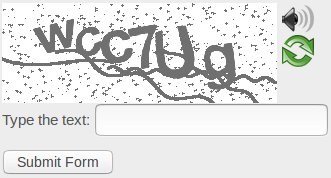
\includegraphics[width=.9\linewidth]{figuras/captcha_letras.png}
		\caption{Letras}
	\end{subfigure}
	\begin{subfigure}{.5\textwidth}
		\centering
		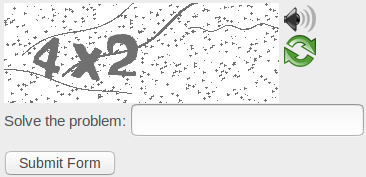
\includegraphics[width=.9\linewidth]{figuras/captcha_mat.png}
		\caption{Desafio matemático}
	\end{subfigure}%
	\vspace{.05\linewidth}
	\begin{subfigure}{.5\textwidth}
		\centering
		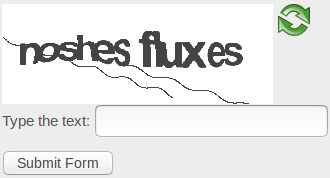
\includegraphics[width=.9\linewidth]{figuras/captcha_texto.png}
		\caption{Duas palavras}
	\end{subfigure}
	\begin{subfigure}{.5\textwidth}
		\centering
		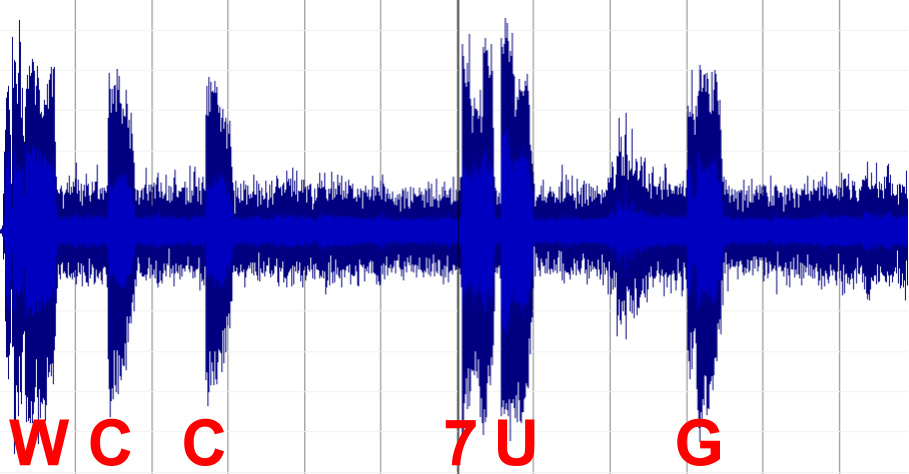
\includegraphics[width=.9\linewidth]{figuras/captcha_audio2.png}
		\caption{Áudio}
	\end{subfigure}
	\caption{Diferentes tipos de CAPTCHAs}
	\small (a) O desafiado deve reconhecer corretamente um texto formado por caracteres não correlacionados. (b) O desafio consiste em extrair e resolver corretamente um problema simples de álgebra. (c) Identificar palavras sorteadas de um repositório. (d) O desafio consiste com extrair corretamente um conjunto de símbolos codificados em áudio. Todos os exemplos foram gerados com a biblioteca Securimage. O espectro de intensidades em (d) foi gerado pelo autor a partir do áudio gerado pela biblioteca.
	\label{diffcaptchas}
\end{figure}

O processo de '\textit{quebra}' envolve duas ideias principais: explorar vulnerabilidades e/ou uso de algoritmos inteligentes. Por serem testes automatizados, CAPTCHAs geralmente apresentam algum padrão de comportamento ou falha de projeto. A padronização na geração de desafios pode permitir que um atacante desenvolva heurísticas de ataque. Imagens com mesmo espaçamento de caracteres ou padrões repetitivos podem ser explorados e facilitar a segmentação da imagem, como foi explorado por \cite{naivecaptcha}. Falhas ou vieses no projeto desses métodos também podem expor brechas. Quanto ao uso de algoritmos inteligentes, redes neurais recebem um lugar de destaque devido a flexibilidade e capacidade de generalização que esses modelos conseguem alcançar. O uso dessa classe de algoritmos foi a abordagem escolhida por \cite{captcha_break_2013} e \cite{lectures2005HIP}, por exemplo. Redes neurais são exploradas no capítulo \ref{cap:neurais}.

Ao longo dos anos os domínio e os desafios tem evoluído em complexidade, na medida que os atacantes evoluem em técnicas de ataque. Um exemplo da co-evolução desses sistemas é a forma como o sistema reCaptcha \cite{recaptcha1} tem mudado ao longo dos anos. Quando proposto, o sistema era baseado em trechos de livros e jornais antigos em que os melhores algoritmos conhecidos à época falharam em uma tarefa de OCR (do inglês optical character recognition). Trechos que não haviam sido corretamente identificados (teste) eram separados e exibidos para humanos juntamente com imagens cuja a extração era reconhecida (controle). Teste e controle eram comparados para certificar a atuação humana. Quando proposto, os autores alegaram que humanos seriam capazes de resolver o desafio em quase todos os casos e que comutadores teriam chance quase nula de passarem desapercebidos, já que o repositório de exemplos era composta por imagens em que as técnicas vigentes à época haviam falhado. Porém, poucos anos depois, avanços em técnicas de OCR baseadas em redes neurais obtiveram $99\%$ de precisão na base de palavras utilizada por esse sistema \cite{captcha_break_2013}, inviabilizando o uso dessa técnica e forçando o reCaptcha a evoluir para uma segunda versão. Nessa nova abordagem, os dados de navegação dos usuários são analisados por um algoritmo de risco. Caso uma pontuação mínima seja atingida, o usuário é considerado humano, caso contrário, é exposto a problemas conhecidamente difíceis para computadores, como reconhecimento de objetos, contextualização de imagens e busca de similaridades, combinados com diferentes ações que devem ser performadas pelo usuário. Entretanto, Sivakorn \textit{Et al.} \cite{imarobot} mostraram que explorando-se os critérios de avaliação de risco, seria possível enganar o sistema em $85\%$ das vezes, forçando a constante atualização dos desafios.

\section{Captchas de texto}\label{sec:captchatexto}

Nos CAPTCHAs baseados em texto, uma imagem contendo uma sequência de caracteres é exibida ao desafiado. O teste consiste em conseguir recuperar corretamente o texto codificado na imagem. Matematicamente, uma imagem com altura $A$, largura $L$ e $C$ canais pode ser representada como um tensor $x \in \Re^{A,L,C}[0,1]$, de modo que  $x_{ijk}$ representa a intensidade do pixel na posição $(i,j)$ canal $k$. Um token é uma sequencia $u$ sob um alfabeto de símbolos $\Sigma$, podendo o comprimento da sequência ser limitado ou não. Assim, '\textit{quebrar}' um CAPTCHA de texo é encontrar um mapa $f(x) \rightarrow u$ que obtenha uma taxa de acerto maior do que às propostas por \cite{lectures2005HIP}. Um sistema de CAPTCHA torna-se completamente inútil se não conseguir diferenciar humanos de robores.

Quanto à imagem, usualmente são utilizadas adição de ruído, linhas e/ou grades para dificultar o processo de segmentação de caracteres \cite{lectures2005HIP}, bem como efeitos de distorção, corrosão e/ou dilatação, e transformações geométricas como rotação e translação, entre outros. Em desafios mais simplórios o número de canais pode ser reduzido à um, podendo ser representado como uma imagem em tons de cinza. Em desafios mais complexos o espaços de canais é explorado, aumentando algebricamente as possibilidades representação, mantendo, todavia, a factibilidade do desafio para seres humanos, dada nossa facilidade em distinguir cores\footnote{Nem sempre esta afirmação é verdadeira. De fato, pessoas que sofrem da Síndrome de Dalton, o Daltoninsmo, podem ter dificuldades em resolver desafios que explorem diferentes cores. O balanço entre complexidade e inclusão de pessoas com necessidades especiais ainda é uma questão em aberto no projeto de CAPTCHAs.}. É possível explorar imagens sintéticas, geradas de forma automatizada por computadores, ou imagens naturais, como paisagens ou textos em fotos reais. 

Quanto ao texto, diferentes complexidades podem ser adicionadas. Fixadas as demais variáveis, a dificuldade do desafio é usualmente proporcional ao tamanho de alfabeto escolhido. Dentre os mais simples, o conjunto dos números $\Sigma = {0123456789}$ possui apenas dez símbolos. No outro extremo, os logogramas chineses constituem alfabetos com um número indeterminado de símbolos, com as representações mais usuais se limitando a algo em torno de $3000$ caracteres. A tipografia também interfere na dificuldade de resolver um CAPTCHA. Para o mesmo alfabeto $\Sigma$ existem diferentes possibilidades de representação gráfica dos seus caracteres. Fontes regulares tendem a fornecer representações mais simples, com a desvantagem de serem facilmente reconhecíveis por OCR. No outro extremo, fontes simbólicas e caracteres escritos à mão podem representar um grande desafio para máquinas. Quando os símbolos são sorteados de forma aleatória, humanos e máquinas, tipicamente, presenciam maiores dificuldades, dado que cada entrada deve ser reconhecida separadamente (errar o reconhecimento um símbolo significa uma falha completa). Quando sorteamos palavras a partir de um repositório, o desafio se torna mais amigável para humanos, primeiro por termos uma facilidade maior em reconhecer padrões do que especifidades e segundo por nos permitir o uso indireto de outras fontes de conhecimento para a solução do problema. Se soubermos que os textos estão em Português, por exemplo, podemos esperar que nenhuma palavra conterá uma subsequência \textit{tt} (gramaticalmente incorreto) ou que uma vogal será, provavelmente, seguida por uma consoante ou por uma vogal diferente (padrão mais frequente na língua). Entretanto, quando o repositório de palavras é exposto, atacantes podem desenvolver heurísticas para explorar o problema, como um dicionário de palavras ou correção gramatical para aprimorar a eficiência das técnicas. Além disso, repositórios de palavras induzem correlações entre os caracteres, o que limita bastante o espaço de possíveis tokens. 

Ver \cite{bursztein2011text} para um apanhado de CAPTCHAs de texto utilizados pelo mundo e \cite{captcha_review_2017} para uma a evolução desses sistemas ao longo dos anos. Na figura \ref{captchasbrasil} temos alguns exemplos utilizados por instituições brasileiras.

\begin{figure}[ht]
	\begin{subfigure}[t]{.475\textwidth}
		\centering
		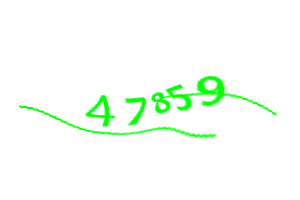
\includegraphics[width=.9\linewidth, height=.4\linewidth]{figuras/captcha_banco_central.png}
		\caption{Banco Central do Brasil}
	\end{subfigure}
	\hspace{.05\textwidth}
	\begin{subfigure}[t]{.475\textwidth}
		\centering
		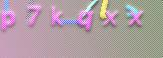
\includegraphics[width=.9\linewidth, height=.4\linewidth]{figuras/captcha_inss.jpeg}
		\caption{Instituto Nacional do Seguro Social (INSS)}
	\end{subfigure}%
	
	\vspace{.05\linewidth}
	\begin{subfigure}[t]{.475\textwidth}
		\centering
		
\includegraphics[width=.9\linewidth, height=.4\linewidth]{figuras/captcha_itau.jpeg}
		\caption{Banco Itaú}
	\end{subfigure}
	\hspace{.05\textwidth}
	\begin{subfigure}[t]{.475\textwidth}
		\centering
		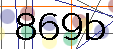
\includegraphics[width=.9\linewidth, height=.4\linewidth]{figuras/captcha_mec.png}
		\caption{ Ministério da Educação (MEC)}
	\end{subfigure}%
	
	\vspace{.05\linewidth}
	\begin{subfigure}[t]{.475\textwidth}
		\centering
		
\includegraphics[width=.9\linewidth, height=.4\linewidth]{figuras/captcha_mprj.jpeg}
		\caption{Ministério Público do Estado do Rio de Janeiro (MPRJ)}
	\end{subfigure}
	\hspace{.05\textwidth}
	\begin{subfigure}[t]{.475\textwidth}
		\centering
		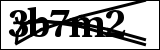
\includegraphics[width=.9\linewidth, height=.4\linewidth]{figuras/captcha_tjpe.png}
		\caption{Tribunal de Justiça do Estado de Pernambuco (TJPE)}
	\end{subfigure}%
	\vspace{.05\linewidth}
	
	\caption{Diferentes CPATCHAs de texto em uso por instituições brasileiras.}
	\small 
	(a) Disponível em: \url{https://www3.bcb.gov.br/faleconosco/#/login/consultar}. Acesso em: 23/06/201.
	(b) Disponível em: \url{https://cadsenha.inss.gov.br/cadsenha-internet-web/faces/pages/segurado/entradaNitNb.xhtml}. Acesso em: 23/06/201. 
	(c) Disponível em: \url{https://bankline.itau.com.br/boletos-novosite/simulador_etapas_boletos_02.htm}. Acesso em: 23/06/201.
	(d) Disponível em: \url{http://painel.mec.gov.br/painel/captcha}. Acesso em: 23/06/201. 
	(e) Disponível em: \url{http://www.mprj.mp.br/comunicacao/ouvidoria/consulte-a-sua-comunicacao}. Acesso em: 23/06/201. 
	(f) Disponível em: \url{https://srv01.tjpe.jus.br/consultaprocessualunificada/}. Acesso em: 23/06/201.
	\label{captchasbrasil}
\end{figure}


\chapter{Redes Neurais} \label{cap:neurais}

Neste capítulo introduziremos redes neurais como uma forma genérica para escrever famílias de funções. Os conceitos de composição, tipos de camadas e arquiteturas são introduzidos. Daremos um enfoque aos dois tipos comuns de camadas que foram usados no presente trabalho. Posteriormente, detalhes técnicos do treino de redes neurais são explorados. 

\section{Introdução}

Dentro do campo de Inteligência Artificial, aprendizado de máquina é uma abordagem algorítmica para inferir regras em um problema a partir de exemplos. Uma categoria especial é a de aprendizado supervisionado, onde os exemplos constituem-se de um \textit{elemento} em um domínio conhecido e um \textit{rótulo} associado. O objetivo é deduzir abstrações que permitam relacionar elementos e rótulos. Nesse contexto, uma rede neural\footnote{Apesar de introduzidas aqui como um algoritmo supervisionado, redes neurais podem ser aplicadas de forma efetiva à problemas não supervisionados.} é, em última análise, uma forma genérica de escrever funções\footnote{Funções estão sendo usadas aqui com um sentido mais relaxado do que o usualmente utilizado na matemática.} sobre relações elemento-rótulo. Dada uma métrica para a estimativa dos erros cometidos por uma relação inferida, o desafio de inferir regras de associação ótimas se torna um problema de encontrar uma função que minimiza nossa estimativa de erro. O adjetivo '\textit{neural}' advém da inspiração em funções biológicas que historicamente influenciaram e ainda influenciam essa forma de exprimir relações. Em resumo, redes neurais são um conjunto de técnicas inspiradas em processos cognitivos desempenhados pelo sistema nervoso que fornecem uma maneira genérica de descrever famílias de funções.

De forma mais específica, dado um conjunto de exemplos $D = \{(x, y)\}$, onde $x$  pertence algum domínio conhecido e $y$ um rótulo associado, desejamos encontrar a função $\hat{y} = f(x)$, de tal modo que $\hat{y}$ seja o mais similar possível à $y$. Por '\textit{mais similar o possível}' entende-se que conhecemos uma estimativa para os erros, também referida como função custo, que é tão menor quanto melhor for a aproximação dada por $f(x)$, e é normalmente representada como $J(y, \hat{y})$. Formalmente, desejamos encontrar $f^*$ tal que
\begin{equation}
f^* = \min_f J^{(D)} = \min_f \langle J(y, f(x)) \rangle_{D},
\end{equation}   
onde $\langle \ldots \rangle_{D}$ representa o valor esperado no conjunto $D$.

Dada uma família de funções $f^{\Theta} : x \rightarrow y$ definida por uma rede neural e parametrizadas por $\Theta$, podemos vasculhar o espaço de busca induzido, $\{\Theta\}$, para encontrar um função que satisfaça alguma propriedade de interesse. Em particular, no caso de aprendizado de máquina, estamos interessados em encontrar o parâmetro $\Theta^*$ tal que:
\begin{equation}\label{thetaotimo}
\Theta^* = \min_{\Theta} \langle J(y, f^{\Theta}(x)) \rangle_{D}.
\end{equation} 

A versatilidade desse formalismo nos permite explorar diferentes tipos de estruturas relacionais. Em particular, relações hierárquicas podem ser emuladas utilizando-se composição de funções. Essa abordagem nos permite construir redes neurais mais complexas e expressivas a partir de unidades básicas mais simples. Neste caso, podemos reescrever a função $f^{\Theta}$ como:
\begin{equation}\label{fcamadas}
f^{\Theta}(x) = f_1^{\Theta_1}(f_2^{\Theta_2} (f_3^{\Theta_3}(\ldots(x))) ),
\end{equation}
sendo $\Theta = (\Theta_1, \Theta_2, \Theta_3, \ldots)$ o parâmetro composto por cada um dos parâmetros individuais.
Quando compomos funções desta forma, é comum nos referirmos à cada função $f_i^{\Theta_i}$ como sendo a $i$-\textit{ésima} \textit{camada} da rede neural, sendo as camadas para além da mais externa também conhecidas como \textit{camadas escondias} (em inglês \textit{hidden layers}). A \textit{profundidade} da rede é uma referência à quantidade de funções internas usadas na composição. Diferentes tipos de funções definem diferentes tipos de transformações, as quais nos referimos como \textit{tipo da camada}. A especificação de todas as camadas em uma rede neural é o que chamamos de \textit{arquitetura} da rede. A seguir vamos explorar dois tipos de camadas que foram utilizados no presente estudo.

\section{Camadas Densas}

Camadas \textit{densas} ou totalmente conectadas definem uma transformação afim entre o conjunto de entradas e saídas. Tipicamente, após a transformação afim, segue-se a aplicação de uma função não linear elemento-à-elemento, conhecida como \textit{função de ativação}, permitindo a expressão de relações mais complexas. As camadas densas são biologicamente inspiradas no mecanismo de comunicação dos neurônios, onde a diferença de potencial elétrico exprimida nas sinapses do axônio é proporcional, em alguma medida, à soma das diferenças de potenciais experimentadas nos dendritos \cite{GerstnerNeuronalDynamics}. As conexões de entrada em um neurônio definem sua regra de ativação, ou seja, quais outros neurônios devem estar ativos (e em que intensidade) para que haja uma transição de estado. Como veremos mais adiante, camadas totalmente conectadas tentam emular o comportamento de vários neurônios simultaneamente.

De maneira mais formal, seja $x$ um vetor no conjunto de entrada, a relação expressa por uma camada densa é dada por:
\begin{equation}\label{denseop}
f^{W,b}(x) = act(W \odot x + b)
\end{equation}
onde $b$ é um vetor, referido como \textit{viés} (ou, no inglês, \textit{bias}), $W$ uma matriz de transformação, $act$ uma função de ativação e $\odot$ é a operação usual de multiplicação de matrizes, definida elemento-à-elemento como $[W \odot x]_{i} = \sum_k W_{ik} * x_k$. Diferentes funções de ativação expressam relações distintas sob um vetor de entrada $z = \{z_i\}$. Dentre os exemplos mais conhecidos na literatura, ressaltamos a função sigmoide, $\sigma(z)_i = \frac{1}{1+\exp(-z_i)}$, que mapeia os elementos de saída no intervalo $\Re[0,1]$, a função de retificação linear (relu), $relu(z)_i = max(0, z_i)$, e a função máximo atenuado (softmax), $\sigma(z)_i = \frac{\exp(z_i)}{\sum_j \exp(z_j)}$, que possui a interessante propriedade $\sum_i \sigma(z)_i = 1$, sendo usualmente utilizada para expressar distribuições de probabilidade.

Podemos interpretar a transformação expressa na equação \ref{denseop} como uma projeção do exemplo $x$ sob um espaço de características que descrevem uma relação que desejamos expressar. De fato, se reescrevermos a $i$-\textit{ésima} linha de $W$ como $\alpha_i \hat{w_i}$, onde $\hat{w_i}$ é um vetor normalizado e $\alpha_i$ a constante de normalização, podemos interpretar cada uma das saídas de uma camada densa (antes da função de ativação) como uma série de projeções balanceadas $\alpha_i \hat{w_i} \odot x + b_i$ ($\odot$ aqui é o produto interno usual). Em outras palavras, a contribuição da $i$-\textit{ésima} saída da camada é dada pela importância $\alpha_i$ dessa característica multiplicada por o quanto do exemplo é composto por essa característica,  $\hat{w_i} \odot x$, adicionado de um viés $b_i$ que independe do exemplo em questão. Assim, para redes densas, determinar os parâmetros ótimos ser entendido como encontrar projeções do espaço de entrada em um conjunto de características que sejam pertinentes ao problema. Neste sentido, cada saída de uma camada densa pode ser interpretada como um neurônio, que exprime em sua saída uma soma balanceada dos estímulos de entrada. Quando compomos camadas densas expressamos características que dependem de outras características. Durante o aprendizado, esperamos que essas projeções sejam descobertas de forma automática pelo modelo. Um desenho esquemático de como essas projeções funcionam pode ser visto na figura \ref{conv_lin}. O número de parâmetros em uma camada densa é dado pelo produto entre tamanho do exemplo de entrada e a quantidade de características.

\begin{figure}[ht!]
	\caption{Imagem ilustrativa das possíveis projeções aprendidas em uma camada (a) densa e (b) convolucional em um problema de reconhecimento de faces.}
	\begin{center}
	\begin{subfigure}{0.6\textwidth}
		\centering
		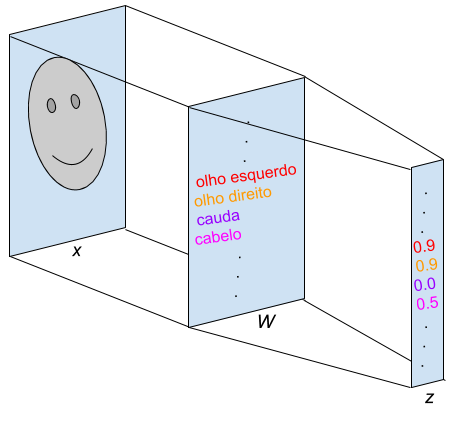
\includegraphics[width=.85\linewidth]{figuras/projlin.png}
		\caption{}
	\end{subfigure}%
	\vspace{.05\linewidth}
	\begin{subfigure}{0.6\textwidth}
		\centering
		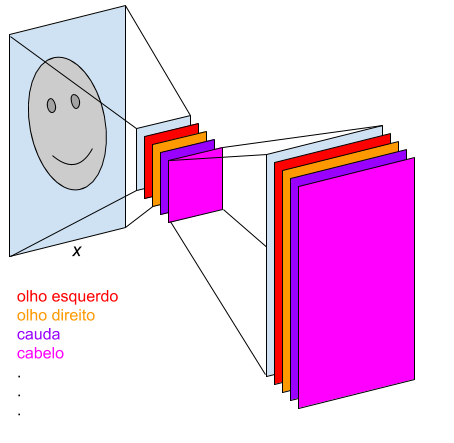
\includegraphics[width=.85\linewidth]{figuras/projcon.png}
		\caption{}
	\end{subfigure}
	\end{center}
	\small Em (a) as projeções atuam sobre todo o exemplo de entrada, mapeando-os em um espaço de importâncias de cada característica. Note que as projeções densas são fixas, no sentido que expressamos '\textit{olho direito}' em uma posição específica. Em (b) expressamos projeções menores que '\textit{varrem}' o exemplo de entrada buscando por uma característica em particular, projetando o exemplo em canais de características. Note que, neste caso, procuramos por uma característica que esteja presente em qualquer lugar da imagem, com os sinais de resposta registrados no canal respectivo. (Fonte: elaborado pelo autor.)
	\label{conv_lin}
\end{figure}


\section{Camadas Convolucionais}

Camadas \textit{convolucionais} \cite{LeCun1989, LeCun98} são similares às densas: definem uma transformação afim representada por uma matriz, seguida, possivelmente, de uma função de ativação. Diferem, entretanto, no tipo de operação matricial utilizada, trocando-se o produto usual de matrizes por uma operação convolucional. Como vimos na seção anterior, cada saída de uma camada densa pode ser interpretada como uma coleção de projeções independentes sob um espaço de características. Em camadas convolucionais, o mesmo operador projeção é reutilizado em diferentes subespaços do conjunto de domínio, varrendo exemplos em busca de padrões específicos, característica usualmente referida como \textit{compartilhamento de parâmetros}. O reuso promove a vantagem de reduzir consideravelmente o espaço de busca $\{\Theta\}$ (Uma imagem ilustrativa do funcionamento dessas camadas pode ser visto na figura \ref{conv_lin}). O número de parâmetros nesse caso é dado pelo produto entre o tamanho da projeção e o número características. Camadas convolucionais são especialmente efetivas quando os elementos do domínio possuem alta localidade, como é o caso de imagens (cada pixel é altamente correlacionado com seus vizinhos em imagens naturais) e séries temporais periódicas (o valor da série do tempo $t$ é correlacionado com o valor da série em $t + \tau$, onde $\tau$ é o período da série). Tipicamente, mais de uma projeção é encapsulada em um mesmo tensor de transformação, sendo a matriz de cada projeção referida como núcleo. O resultado da convolução do núcleo com o exemplo de entrada é tipicamente referida como \textit{canal}.

Matematicamente, dado um tensor $x$ de ranque $3$\footnote{Por simplicidade, estamos definindo aqui a operação de convolução para imagens coloridas, representadas por tensores de ranque $3$. Entretanto, operações de convolução podem ser definidas para outros domínios, como séries temporais (ranque $1$), imagens em tons de cinza (ranque $2$) e vídeo (ranque $4$).}, a atuação da camada de convolução pode ser escrita como
\begin{equation}
f^{W,b}(x) = act(W \otimes x + b)
\end{equation}
onde $W$ é um tensor de transformação que encapsula a informação de diferentes projeções, $b$ é o vetor de viés, de dimensão igual ao número de canais de saída, $act$ uma função de ativação e $\otimes$ é a operação de convolução, definida elemento-à-elemento por
\begin{equation}
[W \otimes x]_{ijd} = \sum_{c} \;\; \sum_{m=i'-k_i}^{i'+ k_i} \sum_{n=j'-k_j}^{j'+k_j} W_{m, n, c, d} * x_{m, n, c}
\end{equation}
onde $c$ ($d$) se estende por todos os canais de entrada (saída), $2k_i+1$ ($2k_j+1$) é o tamanho do núcleo da projeção na direção $i$ ($j$) e a relação $s_i = i'/i$ ($s_j = j'/j$) define o passo da transformação (em geral, $k_i = k_j = k$ e $s_i = s_j = s$). Uma forma intuitiva de visualizar uma operação convolucional é imaginar que a cada etapa $(i,j)$, cada operador de projeção $\tilde{w}$ no tensor $W$ define, por canal, uma região $\tilde{x}$ no tensor de entrada. O resultado da operação de convolução é dado pelo produto interno usual entre $\tilde{w}$ e $\tilde{x}$. No passo seguinte a operação é repetida até que toda a imagem de entrada seja coberta. A contribuição total para cada canal de saída é dado pela soma das convoluções em cada canal de entrada. Um esquema ilustrativo pode ser visto na figura \ref{convw}. 

\begin{figure}[ht]
	\caption{Exemplo esquemático da execução da operação de convolução em um canal do tensor de entrada $x$.}
	\begin{center}
	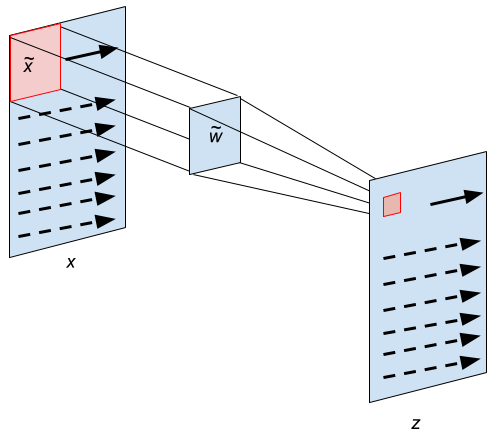
\includegraphics[width=.6\linewidth]{figuras/convwa.png}
	\end{center}
	\small No passo $i,j$, cada operador de projeção $\tilde{w}$ define um campo de atuação $\tilde{x}$. Para o canal $z$, $z_{i,j} = \tilde{w} \odot \tilde{x}$. O produto interno é realizado transformando $\tilde{w}$ em um vetor linha e $\tilde{x}$ em um vetor coluna. (Fonte: elaborado pelo autor.)
	\label{convw}
\end{figure}

Camadas de convolução são inspiradas na interpretação vigente do funcionamento do córtex visual de mamíferos. Diferentes camadas hierárquicas são sensíveis a níveis distintos de abstração na representação de imagens: as iniciais apreendem informações de traços simples, posteriormente composições de traços, formas geométricas, objetos complexos e assim por diante. De fato, estudos mais detalhados das projeções hierárquicas aprendidas por redes convolucionais profundas após o treino mostraram similaridades com o seu análogo biológico \cite{lee2008sparse} e crescentes níveis de abstração na representação das imagens \cite{Gatys2015, gatys2016image}, iniciando com traços simples e texturas nas camadas iniciais e culminando em representações abstratas para objetos nas finais.

Frisamos que esta não é uma lista exaustiva dos diferentes tipos de camada que podem ser encontrados na literatura. Não listadas aqui, mas que merecem destaque, podemos citar redes de capsula \cite{sabour2017dynamic}, que desempenham operações de convolução e posterior alinhamento das ativações dos filtros, e redes recorrentes (e suas variações), que adicionam correlação temporal entre os exemplos através de mecanismos de memória. Uma revisão histórica da evolução dessas camadas pode ser encontrado em \cite{jurgenReview2015}. Para uma descrição mais detalhada das arquiteturas descritas nesse capítulo, incluindo limitações, aplicabilidade e detalhes técnicos, ver \cite{Goodfellow-et-al-2016}.

\section{Aprendizado}\label{sec:aprendizado}

Definida a arquitetura da rede neural, isto é, a sequencia das camadas e respectivas funções de ativação, procedemos para o \textit{treino} da rede, que consiste em encontrar os parâmetros ótimos $\Theta^*$ como definido na equação \ref{thetaotimo}. A forma mais ingenua para procurar o valor ótimo seria utilizar o método do gradiente (ou método do máximo declive), que consiste em atualizar iterativamente $\Theta$ na direção contrária à do gradiente da função custo segundo a regra 
\begin{equation}
\Theta \leftarrow \Theta - l_r \nabla_{\Theta} J^{(D)},
\end{equation}
onde $l_r$ é o \textit{hiper-parâmetro de aprendizado} ou taxa de aprendizado, $D$ o conjunto onde a atualização é realizada e $\nabla_{\Theta}$ o operador gradiente com respeito aos parâmetros $\Theta$. A evolução de $\Theta$ ao longo do treino é referida como \textit{dinâmica do aprendizado}.

O método do gradiente nos garante que, uma vez atingido o mínimo global, o gradiente da função custo é nulo ($\nabla_{\Theta} J^{(D)} = 0$), e nenhuma atualização posterior se fará necessária. Entretanto, não nos é garantido o recíproco: uma vez que $\nabla_{\Theta} J^{(D)} = 0$, não podemos afirmar se encontramos um mínimo local, um ponto de sela ou até mesmo um ponto de máximo. Também não é garantido se eventualmente um ponto de gradiente nulo será encontrado. Adicionalmente, a escolha do hiper-parâmetro $l_r$ e do conjunto de atualização $D$ não são especificados pelo método.

Quanto à escolha do conjunto de atualização, podemos escolher dentre atualizar os parâmetros para cada exemplo, para um subconjunto ou para todos os exemplos disponíveis por vez. No primeiro caso, conhecido como gradiente estocástico, temos a vantagem de atualizar $\Theta$ sempre que a rede é exposta à um exemplo, o que poderia levar á uma convergência mais rápida. Essa escolha é comumente referida como aprendizado \textit{online}. Entretanto, as flutuações estatísticas de cada exemplo podem gerar uma condição de difícil convergência, com o gradiente da função custo mudando drasticamente de direção a cada atualização. No outro extremo, conhecido como gradiente em lote, $D$ constitui todo o conjunto disponível de treino. Nessa escolha, o gradiente em cada exemplo é acumulado e a atualização é feita pela média dos gradientes em todos os exemplos de treino. Apesar da vantagem da estabilidade estatística, corremos dois riscos: demorar demais para atualizar $\Theta$, o que torna o aprendizado mais lento, e a média sobre o conjunto de treino anular ou diminuir particularidades de subconjuntos específicos. Uma terceira opção consiste em juntar o melhor das duas escolhas anteriores: promover a atualização dos parâmetros à cada $N_B$ exemplos. Tal técnica é denominado atualização em mini-lote ou gradiente em mini-lote. E foi a técnica escolhida no presente trabalho.  

Quanto à escolha de $l_r$ temos que buscar um compromisso entre dois extremos. Valores pequenos produzem dinâmicas lentas, onde as atualizações do parâmetros são pequenas e o tempo de treino se estende por diversas iterações. Em alguns casos, a dinâmica pode ficar presa em regiões onde $\nabla_{\Theta} J^{(D)}$ é pequeno mas o valor do custo ainda é alto. No outro extremo, temos uma dinâmica mais rápida, porem mais instável. Pontos de mínimo podem ser completamente ignorados (fenômeno referido como \textit{overshoot}) e a função de erro tende a exibir flutuações que dificultam a convergência. Uma maneira de contornar o problema é utilizar uma abordagem adaptativa. Uma solução simples é diminuir o valor da taxa de aprendizado ao longo do treino, sendo decaimento linear ou exponencial duas escolhas bastante comuns. Dessa forma, temos um balanço entre rápido aprendizado no início da dinâmica e maior estabilidade próximo ao fim. Outras técnicas incluem estabelecer regras de atualização baseadas no gradiente da função de custo e no momento (taxa de atualização do gradiente). A descrição detalhada dessas técnicas fogem ao escopo deste trabalho. Nos experimentos utilizamos a técnica conhecida como Adam \cite{adam_op} que foi especialmente desenvolvida para atualizações em mini-lote e utiliza o momento dos gradientes do custo para estabilizar o aprendizado e decaimento da taxa de treino. Um exemplo esquemático de uma dinâmica lenta ($l_r$ pequeno) e rápida ($l_r$ grande) pode ser vista na figura \ref{convergence}.

\begin{figure}[ht]
	\caption{Exemplo de comportamento característico da função de custo.}
	\begin{center}
	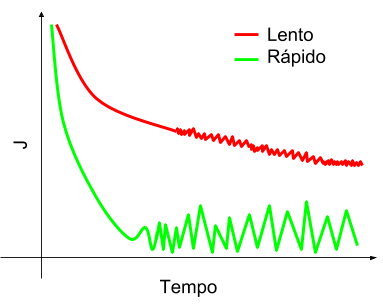
\includegraphics[width=.6\linewidth]{figuras/convergence.png}
	\end{center}
	\small Em vermelho o aprendizado é lento e apresenta flutuações menores. Em verde o custo decai rapidamente, mas apresenta flutuações mais drásticas. (Fonte: elaborado pelo autor.)
	\label{convergence}
\end{figure}


Para redes compostas por várias camadas, como descrito na equação \ref{fcamadas}, a atualização dos parâmetros torna-se complicada e potencialmente suscetível a erros numéricos. Uma forma eficiente de contornar o problema é utilizar a técnica de propagação reversa (em inglês \textit{back-propagation}). Nesta técnica, a computação realizada pela rede é mapeada em um grafo, sendo cada operação realizada na computação expresso como um nó e o fluxo de dados entre duas operações representado por uma aresta direcionada. Durante a fase direta (\textit{feed-foward}) a computação é executada nó-a-nó e os resultados parciais de cada operação armazenados. Durante a fase reversa, as arestas são invertidas e o erro propagado entre os vértices do grafo reverso utilizando-se os valores previamente armazenados e a regra da cadeia para expressar a dependência entre os erros. Durante essa etapa, cada nó que possui um parâmetro a ser aprendido é atualizado. Ver \cite{jurgenReview2015} para uma revisão do método.


\section{Regularização}

Como visto da seção \ref{sec:aprendizado}, durante a evolução da dinâmica de aprendizado, os parâmetros da rede se adaptam de forma a reduzir o valor esperado da função de custo no conjunto de treino. Entretanto, diminuir o erro nos exemplos vistos não garante que o modelo apresentará a mesma qualidade em novos elementos ausentes durante essa fase. De forma mais precisa, seja $U$ o conjunto de todos elemento-rótulo possíveis, tipicamente temos a disposição um subconjunto $D \subset U$ para otimizar a rede, e utilizamos $J^{(D)}$ como um estimador estatístico para $J^{(U)}$, isto é, supondo que $D$ tenha sido formado por instâncias aleatórias de $U$, teremos $J^{(D)} \rightarrow J^{(U)}$ quando $|D| \rightarrow |U|$. Tipicamente, entretanto, temos a situação em que $|D| \lll |U|$. Como o modelo foi otimizado neste subconjunto, o valor esperado da função custo em $D$ se torna um estimador enviesado para o erro esperado em exemplos não vistos. Uma maneira simples e eficiente de estimar a capacidade de generalização modelo é criar a cobertura exata $(D_{tr}, D_{val})$ para $D$, treinar o modelo em $D_{tr}$ e acessar sua qualidade em $D_{val}$. Esta técnica é conhecida como \textit{hold-out}, e $J^{(D_{val})}$ uma estimativa para o poder de generalização do modelo \cite{friedman2001elements}.

Um outro problema recorrente no treino de modelos de aprendizado de máquina é a adequação do modelo ao conjunto de treino. Em um extremo, modelos de baixa expressividade podem não conseguir capturar a complexidade das relações exemplo-rótulo. Esse fenômeno é conhecido como \textit{underfitting}. No outro limite, a medida que aumentamos a expressividade (mais camadas, mais projeções, etc.), aumenta também capacidade de apreender relações mais complexas entre exemplos e rótulos. Entretanto, modelos com maior expressividade tendem a ser mais suscetíveis à '\textit{decorar}' exceções e superestimar particularidades do conjunto de treino. Tal fenômeno é conhecido como coadaptação ou \textit{overfitting}. Outra situação em que podemos incorrer em \textit{overfitting} é quando o modelo é excessivamente exposto aos mesmos exemplos durante uma seção de treino. O \textit{underfitting} pode ser detectado diretamente da qualidade do modelo em $D_{tr}$, quando seu desempenho se mostra aquém do esperado. O segundo pode ser estimado utilizando a decomposição \textit{viés-variância} da estimativa do erro, onde entendemos que parte do erro cometido é devido a baixa expressividade e parte por superestimar particularidades do conjunto de treino. Para tal, a qualidade do modelo em $D_{tr}$ e sua capacidade de generalização (estimada em $D_{val}$) são comparadas e a diferença entre as duas servem para estimar o compromisso entre viés e variância. Um exemplo ilustrativo do comportamento do erro nesses dois conjuntos pode ser visto na figura \ref{overfit}.

\begin{figure}[ht]
	\caption{Exemplo ilustrativo de \textit{overfitting} e \textit{underfitting}.}
 	\begin{center}
	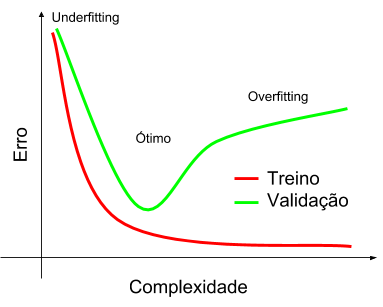
\includegraphics[width=.6\linewidth]{figuras/overfitting.png}
	\end{center}
	\small Em verde vemos que o erro estimado no conjunto de treino se comporta como uma função decrescente da complexidade do modelo. Em vermelho, o erro estimado o conjunto de validação mostra que existe um valor ótimo para o poder de generalização. Fixada a complexidade do modelo, experimenta-se um comportamento similar quando aumentamos a exposição aos exemplos no conjunto de treino. (Fonte: elaborado pelo autor.)
	\label{overfit}
\end{figure}

Para minimizar o efeito de coadaptação dos parâmetros, podemos impor condições extras durante o processo de aprendizado. Uma das condições mais usuais é aplicar ao vetor de parâmetros $\Theta$ alguma restrição. Podemos, por exemplo, adicionar à função custo um termo proporcional à norma do vetor $\Theta$, na forma
\begin{equation}
\tilde{J} = J + \lambda L_n(\Theta),
\end{equation}
onde $\tilde{J}$ é o custo utilizado durante a minimização, $L_n(\Theta) = \sqrt[n]{\Theta^n}$ é a norma $n$ do vetor e $\lambda$ o hiper-parâmetro de regularização ou constante de normalização. Desta forma penalizamos parâmetros que '\textit{aprendam}' demais uma determinada característica. Apesar de efetivo, o uso de regularização baseado em normas adiciona dois novos hiper-parâmetros: a constante de normalização e o tipo de norma que devemos usar. Outra forma de regularização comum na literatura é o \textit{dropout} \cite{hinton2012improving}. Nesta técnica, a saída $i$ de uma camada é removida da computação (atribuída o valor zero) com uma probabilidade $p$, hiper-parâmetro da técnica. Intuitivamente, o uso do \textit{dropout} durante o treino força a rede a aprender representações redundantes e mais robustas à detalhes, dado que a cada nova iteração uma característica aprendida anteriormente pode estar ausente.



\section{Redes Neurais e CAPTCHAs}

Como visto na secção \ref{sec:captchatexto}, CAPTCHAs de texto podem ser vistos como um problema de extração de texto em imagens, sendo assim uma generalização para o problema de OCR e um subproblema de localização de texto em imagens (identificar, se existir, a localização de todos os textos em uma imagem). É preciso ressaltar, entretanto, que nesses HIPs as imagens são especialmente desenvolvidas para serem de difícil solução para computadores e preferencialmente fáceis para seres humanos. Assim, algoritmos usuais de OCR tendem a demonstrar baixo desempenho na solução desses desafios. Vamos separas as abordagens para o problema em dois grandes grupos: abordagens \textit{informadas} e não \textit{informadas}.

Em abordagens informadas o autor do ataque estuda os efeitos e o alfabeto utilizado na confecção do desafio e confecciona um pipeline para preprocessamento e segmentação dos caracteres componentes do token. Esta etapa envolve engenharia reversa e é extremamente dependente da regularidade das imagens para que bons resultados sejam alcançados\footnote{Isso é tipicamente verdade quando a imagem é gerada automaticamente por um computador. Neste caso, técnicas de engenharia reversa podem guiar o desenvolvimento de heurísticas.}. Após a segmentação, o desafio se resume à reconhecer corretamente cada símbolo. Um dos trabalhos pioneiros na quebra de CAPTCHAs de texto foi conduzido por \cite{lectures2005HIP} utilizando-se essa abordagem. Para o reconhecimento foram usadas redes convolucionais de duas camadas, alcançando acurácias entre $10\%$ e $50\%$ (fortemente dependente da qualidade do preprocessamento). Bursztein \textit{et al.} formalizaram ainda mais o pipeline de processamento, lançando a ferramenta \textit{Decaptcha} \cite{bursztein2011text}, que permite explorar e testar etapas do processo de quebra especificando-se técnicas de preprocessamento, segmentação, pos-segmentação, reconhecimento e aprimoramento pós reconhecimento. Com o auxilio da ferramenta, as autores relataram modelos com precisão perfeitas para desafios mais simples. Entretanto, como sugerido pelos próprios autores, a ferramente utiliza na fase de reconhecimento algoritmos com baixo poder de expressividade (k-vizinhos mais próximos e máquinas de vetores de suporte), se comparados com as técnicas modernas. De fato, no repositório do MNIST\footnote{O MNIST (Modified National Institute of Standards and Technology database) é um repositório aberto contendo 70000 imagens de dígitos escritos à mão e usualmente usado como benchmark para técnicas de OCR. A tarefa consiste em reconhecer corretamente o número codificado na imagem. No sítio do repositório existe uma tabela comparativa da precisão de diversos estudos publicados utilizando-se diferentes técnicas ao longo dos anos.} \cite{yann1998mnist}, por exemplo, redes convolucionais pontuam entre as melhores taxas de acerto, sendo o melhor modelo registrado o desenvolvido por {Cire{\c s}an} \textit{et al.}, que alcançou $99.77\%$ de acerto e é baseado na média do voto de 35 redes convolucionais independentes \cite{ciresan2012column}. Outra limitação dessa abordagem é para CAPTCHAs de texto formados por imagens reais, onde as diversas condições de aquisição (iluminação, ângulo, escala, etc.), degradam as vantagens de um pipeline único de preprocessamento. Mesmo neste caso, redes neurais ainda são capazes de demonstrar bom desempenho. Netzer \textit{et al.} propuseram o repositório SVHN\footnote{SVHN (Street View House Numbers), composto por mais de 600000 fotos de fachadas de construções contendo números. O desafio consistem em reconhecer corretamente as algarismos codificados na imagem. O repositório possuem dois formatos para os mesmas imagens: a) Caracteres segmentados; e b) Apenas a região contendo os números.} como benchmark para esse tipo de desafio \cite{netzer2011reading}. Partindo das imagens já segmentadas, os autores foram capazes de obter precisões em torno de $90\%$ utilizando-se abordagens não supervisionadas de redes neurais. O resultado foi posteriormente refinado utilizando-se redes convolucionais profundas e treino supervisionado, alcançando $94.5\%$ de precisão \cite{sermanet2012convolutional}.

Quanto as abordagens não informadas, o modelo deve aprender de forma autônoma como localizar, segmentar e reconhecer os caracteres em uma imagem, minimizando a interferência direta humana. Entretanto, inferir esse nível de abstração apenas baseado em exemplos pode requerer quantidades massivas de dados anotados. Utilizando uma abordagem não informada, Goodfellow \textit{et al.} foram capazes que \cite{captcha_break_2013} de obter $99.8\%$ de acerto nos textos da primeira versão do reCAPTCHA. Os autores ainda conduziram um estudo no repositório SVHN, obtendo acertos de $97.84\%$ por caractere e $96\%$ para o token completo. Entretanto, a base de treino utilizada era formada por 600 mil imagens para o SVHN (toda a base de teino) e mais de um milhão de imagens para o reCaptcha. Em um estudo similar ao nosso, Pinto alcançou $76,6\%$ de precisão na quebra CAPTCHAs utilizando redes neurais profundas. Contudo, foi necessária uma base de treino com 180 mil imagens e placas de processamento gráfico de última geração, sendo o treino realizado em sistemas de computação sob demanda \cite{otaro}. Mais recentemente, foi investigada uma alternativa para diminuir volume de dados necessário para esse tipo de abordagem através de uma nova arquitetura denominada Redes Corticais Recorrentes (do inglês, Recurrent Cortical Network) \cite{captcha_break_2017}. Os atores do estudo relatam resultados próximos ao estado da arte utilizando-se apenas algumas milhares ou até mesmo centenas de imagens de treino. O diferencial dessa arquitetura são conexões extras adicionadas entre as camadas que permite um fluxo mais complexo da informação. Aplicada à quebra de CAPTCHA, os autores treinaram esse tipo de rede em imagens contendo diferentes fontes tipográficas para o mesmo alfabeto. Durante a validação a arquitetura de mostrou capaz de generalizar e abstrair as transformações aplicadas em CAPTCHAs sintéticos, sendo capaz de reconhecer os símbolos mesmo após as deformações. Um ponto negativo, entretanto, é o tempo de treino dessa nova arquitetura. As mensagens trocadas entres as camadas e o algoritmo proposto para supressão de característica limitam a capacidade de paralelização e tornam a execução mais lenta. De fato, há uma nota no repositório dos autores informando que o treino em 1000 imagens do desafio MNIST (onde o algoritmo de aproxima do estado da arte nesse desafio) pode levar horas em múltiplas CPUs\footnote{Fonte: \url{https://github.com/vicariousinc/science_rcn}. Acesso em: 23/06/2018.}. Adicionalmente, os autores alegam que fizeram ajustes nos filtros convolucionais e nas fontes de treino para cada aplicação, o que pode ser interpretado com uma forma de adicionar viés ao modelo (algo como uma abordagem semi-informada).  

Apesar da qualidade dos resultados encontrados na literatura, os requisitos desses sistemas tornam-os proibitivos para o uso em computadores comuns. Na tabela \ref{tableredes} apresentamos um breve comparativo dos requisitos de alguns dos estudos selecionados. Essas restrições limitam o acesso dessa tecnologia à ambientes com menor poder de processamento ou restrições orçamentárias. É particularmente proibitivo para o estudante médio brasileiro, o que pode gerar uma defasagem de aprendizado tecnológico, e para pequenas empresas experimentarem soluções inovadoras baseadas nessas descobertas. Assim, o objetivo deste trabalho é propor um abordagem construtiva para a experimentação de redes neurais profundas focada no problema de \textbf{quebra não informada de CAPTCHAs de texto}. Pretendemos mostrar que é possível alcançar resultados próximos ao estado da arte a partir da investigação cautelosa do comportamento dos modelos ao durante a dinâmica de treino, com bases de treinos menores e arquiteturas mais simples. 


\begin{table}[ht]
\begin{center}
	\begin{tabular}{ c | >{\centering\arraybackslash}m{7cm}  }
		Referência & Limitação  \\ %\hline
		\hline
		Netzer \textit{et al.}     \cite{netzer2011reading}         &  600 mil imagens, 500 filtros convolucionais 8x8.  \\ \hline
		Sermanet \textit{et al.}   \cite{sermanet2012convolutional} &  16 filtros 5x5, 512 filtros 7x7, 2 camadas densas. \\ \hline
		Goodfellow \textit{et al.} \cite{captcha_break_2013}        &  De 9 a 11 camadas convolucionais (8-192 filtros), camada densa com mais de 3 mil entradas, mais de 500 mil exemplos.   \\ \hline
		Pinto \cite{otaro}											& 180 mil exemplos, quatro camadas convolucionais com 64, 128, 256 e 512 canais, duas camadas densas com mais de 4000 entradas.\\ \hline
		Dileep \textit{et al.} \cite{captcha_break_2017}			& Treinameto de difícil paralelização. Muitas horas de treino para alcançar resultados satisfatórios.\\ \hline
\end{tabular}
	\caption{Comparação entre os requisitos dos modelos encontrados na literatura.}
	\label{tableredes}
\end{center}
\end{table}

\chapter{Modelagem}\label{modelagem}



definição das redes
definição da nomenclatura
 

\chapter{Metodologia}

\section{Geração dos CAPTCHAS}

foram geradas 30000 imagens usando diferentes efeitos e cores com tokens de comprimento fixo em 5 utilizando-se a biblioteca \cite{simplecaptcha}

um exemplo constitui de um tensor $(200, 50, 3)$ e de um token $(5, 36)$

exemplos normalizados entre 0-1, token codificado one-hot, de modo que 

\begin{equation}
   p(y[i]|x)= 
	\begin{cases}
		1,	& \text{if } y[i]=w_i\\
		0,  & \text{caso contrário.}
	\end{cases}
\end{equation}

Os 30000 exemplos foram separados, de forma aleatória, em dois conjuntos:
o conjunto de treino, $D_{tr}$, e o de validação, $D_{va}$, com 20000 e 10000 exemplos, respectivamente.

\begin{figure}[ht]
	\begin{subfigure}{.5\textwidth}
		\centering
	 	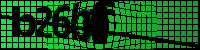
\includegraphics[width=.9\linewidth]{figuras/7103_b26bf.png}
		\caption{b26bf}
	\end{subfigure}
	\begin{subfigure}{.5\textwidth}
		\centering
		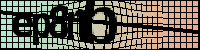
\includegraphics[width=.9\linewidth]{figuras/9456_ep8nb.png}
		\caption{ep8nb}
	\end{subfigure}%
	\vspace{.05\linewidth}

	\begin{subfigure}{.5\textwidth}
		\centering
		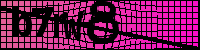
\includegraphics[width=.9\linewidth]{figuras/21856_b7rw8.png}
		\caption{b7rw8}
	\end{subfigure}
	\begin{subfigure}{.5\textwidth}
		\centering
		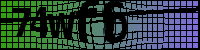
\includegraphics[width=.9\linewidth]{figuras/19816_74wf6.png}
		\caption{74wf6}
	\end{subfigure}%
	\vspace{.05\linewidth}

	\begin{subfigure}{.5\textwidth}
		\centering
		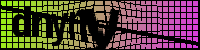
\includegraphics[width=.9\linewidth]{figuras/12248_dnyny.png}
		\caption{dnyny}
	\end{subfigure}
	\begin{subfigure}{.5\textwidth}
		\centering
		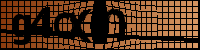
\includegraphics[width=.9\linewidth]{figuras/8873_g4cxh.png}
		\caption{g4cxh}
	\end{subfigure}%
	\vspace{.05\linewidth}

	\caption{Exemplos de CAPTCHAS gerados e seus respectivos tokens.}
\end{figure}



\section{Grandezas de interesse}

\begin{equation}
	S_i^{(D)} = \sum_{(x,y) \in D} p(y[i]|x) \log \hat{p}(y[i]|x)
\end{equation}

\begin{equation}
	acc_w^{(D)} = \frac{N_w}{|D|}
\end{equation}

\begin{equation}
\hat{p}_i^{(D)} = acc_i^{(D)} = \frac{N_i}{|D|}
\end{equation}

\begin{equation}
\hat{p_w}^{(D)} = \prod_{i} \hat{p}_i^{(D)}
\end{equation}

\begin{equation}
loss_i^{(D)} = \frac{S_i}{|D|}
\end{equation}

\begin{equation}
loss^{(D)} = \sum_{i} loss_i^{(D)}
\end{equation}

$t$ tempo total de execução de uma época (treino + validação)
$\tilde{t}$ tempo de treino em uma época.

\section{Treino e Validação}

Todos as redes foram treinadas em um mesmo computador com pentium core i5, 8gb de ram usando tensorflow.

Redes inicializadas segundo critério de \cite{xavier_init}

etapa de treino consiste em
mini batch: sortear $D_{batch} \subset  D_{tr}$, com $|D_{batch}| = 10$ e minimizar  $S_i$'s nesse conjunto usando com \cite{adam_op} com taxa de aprendizado $l_r$. 

O treino em uma época consiste em repetir $|D_{tr}|/|D_{batch}|$ vezes.

calcular as grandezas de interesse em $D_{tr}$ e $D_{va}$


experimentos realizados com diferentes taxas de aprendizado durante 10 épocas. Limite superior e inferior escolhidos manualmente baseados em melhor desempenho aprendizado rápido para a superior e estável para a inferior. Decaimento linear.

Treinado usando critério de parada: mínimo de 10 épocas, máximo de 50 épocas, custo no conjunto de validação na época atual não maior que o .10 do menor valor encontrado até agora, custo no conjunto de treinamento atual menor que .03 da média dos últimos 5 valores. Inspirado em \cite{lutz_early_stop}

\chapter{Resultados} \label{resultados}




\cite{otaro}
5x5 k64, 5x5 e 128, 5x5 e 256, 3x3k512, 16896x4096 dense, 5 camadas densas 4096x36. alcança 76,6 no teste, 95,3 no treino

\chapter{Conclusões}

Neste trabalho propomos uma abordagem comparativa entre diferentes arquiteturas de redes neurais para a solução de CAPTCHAs baseados em texto sem informação humana em um ambiente com capacidade computacional inferior às comumente encontradas na literatura. Mostramos que é possível obter performances próximas ao estado da arte a despeito das limitações. O modelo final escolhido obteve uma acuráciafinal de $96.06\%$ de acerto por token, utilizando menos parâmetros, com requisitos de tempo factíveis e treinado em um mero computador pessoal. Seguem nossas observações para que esse tipo de resultado possa ser reproduzido em outras aplicações.

A experimentação dos hiper-parâmetros é um fator chave na obtenção de bons resultados. Como mostrado pelos experimentos, diferentes configurações do hiper-parâmetro de aprendizado podem levar a dinâmicas de treino substancialmente diferentes. Adicionalmente, diferentes arquiteturas possuem diferentes requisitos. É possível projetar arquiteturas que atendam diferentes especificações (tempo de treino, tamanho, acurácia, etc.) e escolher dentre elas a que melhor se aplica ao problema. Para tal, a análise da dinâmica inicial da rede e o uso de validação cruzada são essenciais. Em particular, a avaliação comparativa da evolução da função custo fornece informação crucial para a escolha e projeto de modelos melhores. Escolhido cuidadosamente uma arquitetura que atenda aos requisitos e os valores ideais para os hiper-parâmetros, é possível realizar seções de treino mais longas, com uma maior exposição do modelo à base de treino e refinar ainda mais os resultados. 

Arquiteturas convolucionais mostraram-se extremamente eficazes para o problema. De fato, esse tipo de camada tem sido aplicada com sucesso em diversos problemas de processamento de imagem. O compartilhamento de parâmetros ao mesmo tempo reduz o tamanho e adiciona maior poder de expressão aos modelos. O \textit{dropout} mostrou-se uma ferramenta eficaz e computacionalmente barata para combater o \textit{overfitting}, melhorando a performance dos modelos estudados sem degradação preceptiva no tempo de computação. A operação de agrupamento com valor fixo apresentou desempenho superior à de \textit{maxout}, tanto no requisito de tempo quanto na acurácia final dos modelos.

\section{Trabalhos futuros}

Segue uma lista de trabalhos futuros que podem enriquecer a discussão iniciapa pelo presente trabalho.

\begin{enumerate}
	\item Explorar mais detalhadamente a influência do número de canais e do tamanho dos núcleos das camadas convolucionais no desempenho das redes, buscando tanto diminuir o número de parâmetros quanto aumentar a acurácia final dos modelos.
	\item Aplicar a mesma abordagem à outros problemas de processamento de imagem, como detecção de objetos, por exemplo, ou outras áreas como predição de sequências temporais.
	\item Estender os modelos os modelos para CAPTCHAs com palavras de sequência variável e/ou diferentes formatos.
	\item Utilizar as mesmas técnicas em CAPTCHAs de texto reais. Em particular, avaliar qual o nível de segurança que esses mecanismos de proteção tem fornecido a instituições no Brasil  
\end{enumerate}


% ----------------------------------------------------------
% ELEMENTOS PÓS-TEXTUAIS
% ----------------------------------------------------------
\postextual
% ----------------------------------------------------------

% ----------------------------------------------------------
% Referências bibliográficas
% ----------------------------------------------------------
\bibliography{referencias.bib}


%---------------------------------------------------------------------
% INDICE REMISSIVO
%---------------------------------------------------------------------
\phantompart
\printindex
%---------------------------------------------------------------------

\appendix


\chapter{Configurações com $l_r = 10^{-3} \;\; \text{e} \;\; 10^{-4}$ na décima época.}\label{cap:apendiceA}

\begin{tiny}

\begin{table}[H]
	\begin{center}
		\begin{tabular}{ |c|c|c|c|c|c|c| }
			
			\hline
			\multirow{2}{*}{modelo} & 
			\multirow{2}{*}{$l_r$} & 
			\multicolumn{2}{c|}{$D_{tr}$} &
			\multicolumn{2}{c|}{$D_{val}$} &
			\multirow{2}{*}{$\frac{J^{(D_{val})}}{J^{(D_{tr})}} - 1$}   \\ \cline{3-6}
			&  & $J$ & $\hat{p}_u$ & $J$ & $\hat{p}_u$  &  \\[2pt]
			
\hline
\multirow{2}{*}{$M$}
& $10^{-3}$ & $1.81\,10^{-1}$ & $0.37$ & $3.98\,10^{-1}$ & $0.21$ & $1.20$ \\ \cline{2-7}
& $10^{-4}$ & $4.77\,10^{-2}$ & $0.53$ & $9.34\,10^{-2}$ & $0.30$ & $0.96$ \\ \cline{2-7}
\hline\hline
\multirow{2}{*}{$MD$}
& $10^{-3}$ & $1.50\,10^{-1}$ & $0.44$ & $3.31\,10^{-1}$ & $0.26$ & $1.20$ \\ \cline{2-7}
& $10^{-4}$ & $7.59\,10^{-2}$ & $0.49$ & $1.17\,10^{-1}$ & $0.35$ & $0.55$ \\ \cline{2-7}
\hline\hline
\multirow{2}{*}{$C_6M$}
& $10^{-3}$ & $2.88\,10^{-3}$ & $0.96$ & $1.20\,10^{-1}$ & $0.49$ & $40.49$ \\ \cline{2-7}
& $10^{-4}$ & $2.41\,10^{-2}$ & $0.74$ & $7.34\,10^{-2}$ & $0.41$ & $2.05$ \\ \cline{2-7}
\hline\hline
\multirow{2}{*}{$C_6MD$}
& $10^{-3}$ & $2.80\,10^{-3}$ & $0.96$ & $6.56\,10^{-2}$ & $0.56$ & $22.40$ \\ \cline{2-7}
& $10^{-4}$ & $3.27\,10^{-2}$ & $0.72$ & $6.02\,10^{-2}$ & $0.51$ & $0.84$ \\ \cline{2-7}
\hline\hline
\multirow{2}{*}{$C_6MMax$}
& $10^{-3}$ & $2.26\,10^{-3}$ & $0.97$ & $1.01\,10^{-1}$ & $0.54$ & $43.56$ \\ \cline{2-7}
& $10^{-4}$ & $1.93\,10^{-2}$ & $0.79$ & $6.63\,10^{-2}$ & $0.47$ & $2.43$ \\ \cline{2-7}
\hline\hline
\multirow{2}{*}{$C_6C_{12}M$}
& $10^{-3}$ & $2.16\,10^{-3}$ & $0.97$ & $8.50\,10^{-2}$ & $0.64$ & $38.43$ \\ \cline{2-7}
& $10^{-4}$ & $1.45\,10^{-2}$ & $0.81$ & $6.15\,10^{-2}$ & $0.54$ & $3.23$ \\ \cline{2-7}
\hline\hline
\multirow{2}{*}{$C_6C_{12}MD$}
& $10^{-3}$ & $2.33\,10^{-3}$ & $0.96$ & $4.49\,10^{-2}$ & $0.68$ & $18.24$ \\ \cline{2-7}
& $10^{-4}$ & $2.12\,10^{-2}$ & $0.81$ & $4.21\,10^{-2}$ & $0.65$ & $0.99$ \\ \cline{2-7}
\hline\hline
\multirow{2}{*}{$C_6C_{12}MMax$}
& $10^{-3}$ & $3.49\,10^{-3}$ & $0.95$ & $7.89\,10^{-2}$ & $0.64$ & $21.58$ \\ \cline{2-7}
& $10^{-4}$ & $1.24\,10^{-2}$ & $0.83$ & $5.60\,10^{-2}$ & $0.57$ & $3.50$ \\ \cline{2-7}
			\hline\hline
\multirow{2}{*}{$C_6C_{12}Fl_{100}M$}
& $10^{-3}$ & $1.00\,10^{-2}$ & $0.85$ & $6.95\,10^{-2}$ & $0.57$ & $5.95$ \\ \cline{2-7}
& $10^{-4}$ & $3.28\,10^{-2}$ & $0.62$ & $7.07\,10^{-2}$ & $0.40$ & $1.15$ \\ \cline{2-7}
\hline\hline
\multirow{2}{*}{$C_6C_{12}Fl_{100}MD$}
& $10^{-3}$ & $1.99\,10^{-2}$ & $0.74$ & $4.34\,10^{-2}$ & $0.60$ & $1.18$ \\ \cline{2-7}
& $10^{-4}$ & $2.10\,10^{-2}$ & $0.78$ & $4.16\,10^{-2}$ & $0.62$ & $0.98$ \\ \cline{2-7}
\hline\hline
\multirow{2}{*}{$C_6C_{12}Fl_{100}MMax$}
& $10^{-3}$ & $4.88\,10^{-2}$ & $0.46$ & $1.14\,10^{-1}$ & $0.27$ & $1.33$ \\ \cline{2-7}
& $10^{-4}$ & $8.87\,10^{-2}$ & $0.19$ & $1.09\,10^{-1}$ & $0.13$ & $0.23$ \\ \cline{2-7}


\hline
		\end{tabular}\hfill%
\end{center}

\end{table}

\newpage
\section*{(\textit{Continuação})}
%\noindent
%\textit{continuação...}
%\newline
\begin{table}[H]
	\begin{center}
		\begin{tabular}{ |c|c|c|c|c|c|c| }
			
			\hline
			\multirow{2}{*}{modelo} & 
			\multirow{2}{*}{$l_r$} & 
			\multicolumn{2}{c|}{$D_{tr}$} &
			\multicolumn{2}{c|}{$D_{val}$} &
			\multirow{2}{*}{$\frac{J^{(D_{val})}}{J^{(D_{tr})}} - 1$}   \\ \cline{3-6}
			&  & $J$ & $\hat{p}_u$ & $J$ & $\hat{p}_u$  &  \\[2pt]
			
			\hline\hline
			\multirow{2}{*}{$C_6C_{12}C_{36}C_{36}M$}
			& $10^{-3}$ & $4.61\,10^{-3}$ & $0.93$ & $3.19\,10^{-2}$ & $0.80$ & $5.91$ \\ \cline{2-7}
			& $10^{-4}$ & $1.86\,10^{-2}$ & $0.78$ & $4.19\,10^{-2}$ & $0.63$ & $1.26$ \\ \cline{2-7}
			\hline\hline
			\multirow{2}{*}{$C_6C_{12}C_{36}C_{36}MD$}
			& $10^{-3}$ & $6.93\,10^{-3}$ & $0.92$ & $1.61\,10^{-2}$ & $0.86$ & $1.33$ \\ \cline{2-7}
			& $10^{-4}$ & $2.32\,10^{-2}$ & $0.81$ & $2.91\,10^{-2}$ & $0.76$ & $0.25$ \\ \cline{2-7}
			\hline\hline
			\multirow{2}{*}{$C_6C_{12}C_{36}C_{36}MMax$}
			& $10^{-3}$ & $8.19\,10^{-3}$ & $0.89$ & $3.47\,10^{-2}$ & $0.76$ & $3.24$ \\ \cline{2-7}
			& $10^{-4}$ & $1.39\,10^{-2}$ & $0.83$ & $3.58\,10^{-2}$ & $0.71$ & $1.58$ \\ \cline{2-7}
			\hline\hline
			\multirow{2}{*}{$C_6C_{12}C_{36}C_{36}Fl_{100}M$}
			& $10^{-3}$ & $1.02\,10^{-2}$ & $0.86$ & $2.61\,10^{-2}$ & $0.76$ & $1.56$ \\ \cline{2-7}
			& $10^{-4}$ & $1.56\,10^{-2}$ & $0.80$ & $3.46\,10^{-2}$ & $0.67$ & $1.22$ \\ \cline{2-7}
			\hline\hline
			\multirow{2}{*}{$C_6C_{12}C_{36}C_{36}Fl_{100}MD$}
			& $10^{-3}$ & $1.06\,10^{-2}$ & $0.86$ & $1.66\,10^{-2}$ & $0.81$ & $0.57$ \\ \cline{2-7}
			& $10^{-4}$ & $1.81\,10^{-2}$ & $0.81$ & $2.52\,10^{-2}$ & $0.75$ & $0.40$ \\ \cline{2-7}
			\hline\hline
			\multirow{2}{*}{$C_6C_{12}C_{36}C_{36}Fl_{100}MMax$}
			& $10^{-3}$ & $9.67\,10^{-3}$ & $0.87$ & $2.32\,10^{-2}$ & $0.79$ & $1.39$ \\ \cline{2-7}
			& $10^{-4}$ & $1.40\,10^{-2}$ & $0.82$ & $3.21\,10^{-2}$ & $0.70$ & $1.28$ \\ \cline{2-7} \hline
		\end{tabular}\hfill%
	\end{center}
	
\end{table}



\end{tiny}

\chapter{Descrição completa das arquiteturas.}\label{cap:apendice_arquiteturas}

\begin{tiny}

\section*{$M$[D]}

\begin{table}[H]
	$M$ $\tilde{\tau}=726.29 (+0.00\%), \tau=1009.74 (+0.00\%)$\newline
	\begin{tabularx}{\linewidth}{ |c|X|c|c|c| }
		\hline
		Camada & Descrição & Entrada & Saída & Parâmetros \\ \hline
		Lin & \multicolumn{1}{c|}{-} & (50,200,3) & (30000) & 0 \\ \hline
		$M$ & 5 classificadores. & (30000) & (5,36) & 5400000 \\ \hline
		total &  &  &  & 5400000 \\ \hline
	\end{tabularx}
\end{table}

\begin{table}[H]
	$MD$ $\tilde{\tau}=759.56 (+4.58\%), \tau=1081.43 (+7.10\%)$\newline
	\begin{tabularx}{\linewidth}{ |c|X|c|c|c| }
		\hline
		Camada & Descrição & Entrada & Saída & Parâmetros \\ \hline
		Lin & \multicolumn{1}{c|}{-} & (50,200,3) & (30000) & 0 \\ \hline
		Dropout & Dropout com $p_{drop} = 30\%$. & (30000) & (30000) & 0 \\ \hline
		$M$ & 5 classificadores. & (30000) & (5,36) & 5400000 \\ \hline
		total &  &  &  & 5400000 \\ \hline
	\end{tabularx}
\end{table}

\section*{$C_6M$[D][Max]}

\begin{table}[H]
	$C_6M$ $\tilde{\tau}=669.60 (+0.00\%), \tau=912.38 (+0.00\%)$\newline
	\begin{tabularx}{\linewidth}{ |c|X|c|c|c| }
		\hline
		Camada & Descrição & Entrada & Saída & Parâmetros \\ \hline
		$C_{6}$ & Convolucional com 3 canais de entrada e 6 de saída. Passo da transformação 2. & (50,200,3) & (23,98,6) & 450 \\ \hline
		Lin & \multicolumn{1}{c|}{-} & (23,98,6) & (13524) & 0 \\ \hline
		$M$ & 5 classificadores. & (13524) & (5,36) & 2434320 \\ \hline
		total &  &  &  & 2434770 \\ \hline
	\end{tabularx}
\end{table}

\begin{table}[H]
	$C_6MD$ $\tilde{\tau}=711.85 (+6.31\%), \tau=975.67 (+6.94\%)$\newline
	\begin{tabularx}{\linewidth}{ |c|X|c|c|c| }
		\hline
		Camada & Descrição & Entrada & Saída & Parâmetros \\ \hline
		$C_{6}$ & Convolucional com 3 canais de entrada e 6 de saída. Passo da transformação 2. & (50,200,3) & (23,98,6) & 450 \\ \hline
		Lin & \multicolumn{1}{c|}{-} & (23,98,6) & (13524) & 0 \\ \hline
		Dropout & Dropout com $p_{drop} = 30\%$. & (13524) & (13524) & 0 \\ \hline
		$M$ & 5 classificadores. & (13524) & (5,36) & 2434320 \\ \hline
		total &  &  &  & 2434770 \\ \hline
	\end{tabularx}
\end{table}

\begin{table}[H]
	$C_6MMax$ $\tilde{\tau}=1334.50 (+99.30\%), \tau=1652.03 (+81.07\%)$\newline
	\begin{tabularx}{\linewidth}{ |c|X|c|c|c| }
		\hline
		Camada & Descrição & Entrada & Saída & Parâmetros \\ \hline
		$C_{6}$ & Convolucional com 3 canais de entrada e 6 de saída. Passo da transformação 2. Maxout. & (50,200,3) & (23,98,6) & 450 \\ \hline
		Lin & \multicolumn{1}{c|}{-} & (23,98,6) & (13524) & 0 \\ \hline
		$M$ & 5 classificadores. & (13524) & (5,36) & 2434320 \\ \hline
		total &  &  &  & 2434770 \\ \hline
	\end{tabularx}
\end{table}

\section*{$C_6C_{12}M$[D][Max]}

\begin{table}[H]
	$C_6C_{12}M$ $\tilde{\tau}=2138.93 (+0.00\%), \tau=2547.99 (+0.00\%)$\newline
	\begin{tabularx}{\linewidth}{ |c|X|c|c|c| }
		\hline
		Camada & Descrição & Entrada & Saída & Parâmetros \\ \hline
		$C_{6}$ & Convolucional com 3 canais de entrada e 6 de saída. Passo da transformação 1. & (50,200,3) & (46,196,6) & 450 \\ \hline
		$C_{12}$ & Convolucional com 6 canais de entrada e 12 de saída. Passo da transformação 2. & (46,196,6) & (21,96,12) & 1800 \\ \hline
		Lin & \multicolumn{1}{c|}{-} & (21,96,12) & (24192) & 0 \\ \hline
		$M$ & 5 classificadores. & (24192) & (5,36) & 4354560 \\ \hline
		total &  &  &  & 4356810 \\ \hline
	\end{tabularx}
\end{table}

\begin{table}[H]
	$C_6C_{12}MD$ $\tilde{\tau}=2386.58 (+11.58\%), \tau=2910.10 (+14.21\%)$\newline
	\begin{tabularx}{\linewidth}{ |c|X|c|c|c| }
		\hline
		Camada & Descrição & Entrada & Saída & Parâmetros \\ \hline
		$C_{6}$ & Convolucional com 3 canais de entrada e 6 de saída. Passo da transformação 1. & (50,200,3) & (46,196,6) & 450 \\ \hline
		Dropout & Dropout com $p_{drop} = 30\%$. & (46,196,6) & (46,196,6) & 0 \\ \hline
		$C_{12}$ & Convolucional com 6 canais de entrada e 12 de saída. Passo da transformação 2. & (46,196,6) & (21,96,12) & 1800 \\ \hline
		Dropout & Dropout com $p_{drop} = 30\%$. & (21,96,12) & (21,96,12) & 0 \\ \hline
		Lin & \multicolumn{1}{c|}{-} & (21,96,12) & (24192) & 0 \\ \hline
		$M$ & 5 classificadores. & (24192) & (5,36) & 4354560 \\ \hline
		total &  &  &  & 4356810 \\ \hline
	\end{tabularx}
\end{table}

\begin{table}[H]
	$C_6C_{12}MMax$ $\tilde{\tau}=3821.52 (+78.67\%), \tau=4365.97 (+71.35\%)$\newline
	\begin{tabularx}{\linewidth}{ |c|X|c|c|c| }
		\hline
		Camada & Descrição & Entrada & Saída & Parâmetros \\ \hline
		$C_{6}$ & Convolucional com 3 canais de entrada e 6 de saída. Passo da transformação 1. Maxout. & (50,200,3) & (46,196,6) & 450 \\ \hline
		$C_{12}$ & Convolucional com 6 canais de entrada e 12 de saída. Passo da transformação 2. Maxout. & (46,196,6) & (21,96,12) & 1800 \\ \hline
		Lin & \multicolumn{1}{c|}{-} & (21,96,12) & (24192) & 0 \\ \hline
		$M$ & 5 classificadores. & (24192) & (5,36) & 4354560 \\ \hline
		total &  &  &  & 4356810 \\ \hline
	\end{tabularx}
\end{table}

\section*{$C_6C_{12}Fl_{100}M$[D][Max]}

\begin{table}[H]
	$C_6C_{12}Fl_{100}M$ $\tilde{\tau}=2873.60 (+0.00\%), \tau=3219.16 (+0.00\%)$\newline
	\begin{tabularx}{\linewidth}{ |c|X|c|c|c| }
		\hline
		Camada & Descrição & Entrada & Saída & Parâmetros \\ \hline
		$C_{6}$ & Convolucional com 3 canais de entrada e 6 de saída. Passo da transformação 1. & (50,200,3) & (46,196,6) & 450 \\ \hline
		$C_{12}$ & Convolucional com 6 canais de entrada e 12 de saída. Passo da transformação 2. & (46,196,6) & (21,96,12) & 1800 \\ \hline
		Lin & \multicolumn{1}{c|}{-} & (21,96,12) & (24192) & 0 \\ \hline
		$Fl_{100}$ & Camada densa com 24192 sinais de entrada e 100 sinais de saída. & (24192) & (100) & 2419200 \\ \hline
		$M$ & 5 classificadores. & (100) & (5,36) & 18000 \\ \hline
		total &  &  &  & 2439450 \\ \hline
	\end{tabularx}
\end{table}

\begin{table}[H]
	$C_6C_{12}Fl_{100}MD$ $\tilde{\tau}=3114.23 (+8.37\%), \tau=3575.14 (+11.06\%)$\newline
	\begin{tabularx}{\linewidth}{ |c|X|c|c|c| }
		\hline
		Camada & Descrição & Entrada & Saída & Parâmetros \\ \hline
		$C_{6}$ & Convolucional com 3 canais de entrada e 6 de saída. Passo da transformação 1. & (50,200,3) & (46,196,6) & 450 \\ \hline
		Dropout & Dropout com $p_{drop} = 30\%$. & (46,196,6) & (46,196,6) & 0 \\ \hline
		$C_{12}$ & Convolucional com 6 canais de entrada e 12 de saída. Passo da transformação 2. & (46,196,6) & (21,96,12) & 1800 \\ \hline
		Dropout & Dropout com $p_{drop} = 30\%$. & (21,96,12) & (21,96,12) & 0 \\ \hline
		Lin & \multicolumn{1}{c|}{-} & (21,96,12) & (24192) & 0 \\ \hline
		$Fl_{100}$ & Camada densa com 24192 sinais de entrada e 100 sinais de saída. & (24192) & (100) & 2419200 \\ \hline
		$M$ & 5 classificadores. & (100) & (5,36) & 18000 \\ \hline
		total &  &  &  & 2439450 \\ \hline
	\end{tabularx}
\end{table}

\begin{table}[H]
	$C_6C_{12}Fl_{100}MMax$ $\tilde{\tau}=4563.22 (+58.80\%), \tau=5045.06 (+56.72\%)$\newline
	\begin{tabularx}{\linewidth}{ |c|X|c|c|c| }
		\hline
		Camada & Descrição & Entrada & Saída & Parâmetros \\ \hline
		$C_{6}$ & Convolucional com 3 canais de entrada e 6 de saída. Passo da transformação 1. Maxout. & (50,200,3) & (46,196,6) & 450 \\ \hline
		$C_{12}$ & Convolucional com 6 canais de entrada e 12 de saída. Passo da transformação 2. Maxout. & (46,196,6) & (21,96,12) & 1800 \\ \hline
		Lin & \multicolumn{1}{c|}{-} & (21,96,12) & (24192) & 0 \\ \hline
		$Fl_{100}$ & Camada densa com 24192 sinais de entrada e 100 sinais de saída. & (24192) & (100) & 2419200 \\ \hline
		$M$ & 5 classificadores. & (100) & (5,36) & 18000 \\ \hline
		total &  &  &  & 2439450 \\ \hline
	\end{tabularx}
\end{table}

\section*{$C_6C_{12}C_{36}C_{36}M$[D][Max]}

\begin{table}[H]
	$C_6C_{12}C_{36}C_{36}M$ $\tilde{\tau}=2191.11 (+0.00\%), \tau=2580.79 (+0.00\%)$\newline
	\begin{tabularx}{\linewidth}{ |c|X|c|c|c| }
		\hline
		Camada & Descrição & Entrada & Saída & Parâmetros \\ \hline
		$C_{6}$ & Convolucional com 3 canais de entrada e 6 de saída. Passo da transformação 1. & (50,200,3) & (46,196,6) & 450 \\ \hline
		$C_{12}$ & Convolucional com 6 canais de entrada e 12 de saída. Passo da transformação 2. & (46,196,6) & (21,96,12) & 1800 \\ \hline
		$C_{36}$ & Convolucional com 12 canais de entrada e 36 de saída. Passo da transformação 2. & (21,96,12) & (9,46,36) & 10800 \\ \hline
		$C_{36}$ & Convolucional com 36 canais de entrada e 36 de saída. Passo da transformação 2. & (9,46,36) & (3,21,36) & 32400 \\ \hline
		Lin & \multicolumn{1}{c|}{-} & (3,21,36) & (2268) & 0 \\ \hline
		$M$ & 5 classificadores. & (2268) & (5,36) & 408240 \\ \hline
		total &  &  &  & 453690 \\ \hline
	\end{tabularx}
\end{table}

\begin{table}[H]
	$C_6C_{12}C_{36}C_{36}MD$ $\tilde{\tau}=2495.31 (+13.88\%), \tau=3024.40 (+17.19\%)$\newline
	\begin{tabularx}{\linewidth}{ |c|X|c|c|c| }
		\hline
		Camada & Descrição & Entrada & Saída & Parâmetros \\ \hline
		$C_{6}$ & Convolucional com 3 canais de entrada e 6 de saída. Passo da transformação 1. & (50,200,3) & (46,196,6) & 450 \\ \hline
		Dropout & Dropout com $p_{drop} = 30\%$. & (46,196,6) & (46,196,6) & 0 \\ \hline
		$C_{12}$ & Convolucional com 6 canais de entrada e 12 de saída. Passo da transformação 2. & (46,196,6) & (21,96,12) & 1800 \\ \hline
		Dropout & Dropout com $p_{drop} = 30\%$. & (21,96,12) & (21,96,12) & 0 \\ \hline
		$C_{36}$ & Convolucional com 12 canais de entrada e 36 de saída. Passo da transformação 2. & (21,96,12) & (9,46,36) & 10800 \\ \hline
		Dropout & Dropout com $p_{drop} = 30\%$. & (9,46,36) & (9,46,36) & 0 \\ \hline
		$C_{36}$ & Convolucional com 36 canais de entrada e 36 de saída. Passo da transformação 2. & (9,46,36) & (3,21,36) & 32400 \\ \hline
		Dropout & Dropout com $p_{drop} = 30\%$. & (3,21,36) & (3,21,36) & 0 \\ \hline
		Lin & \multicolumn{1}{c|}{-} & (3,21,36) & (2268) & 0 \\ \hline
		$M$ & 5 classificadores. & (2268) & (5,36) & 408240 \\ \hline
		total &  &  &  & 453690 \\ \hline
	\end{tabularx}
\end{table}

\begin{table}[H]
	$C_6C_{12}C_{36}C_{36}MMax$ $\tilde{\tau}=5099.87 (+132.75\%), \tau=5718.50 (+121.58\%)$\newline
	\begin{tabularx}{\linewidth}{ |c|X|c|c|c| }
		\hline
		Camada & Descrição & Entrada & Saída & Parâmetros \\ \hline
		$C_{6}$ & Convolucional com 3 canais de entrada e 6 de saída. Passo da transformação 1. Maxout. & (50,200,3) & (46,196,6) & 450 \\ \hline
		$C_{12}$ & Convolucional com 6 canais de entrada e 12 de saída. Passo da transformação 2. Maxout. & (46,196,6) & (21,96,12) & 1800 \\ \hline
		$C_{36}$ & Convolucional com 12 canais de entrada e 36 de saída. Passo da transformação 2. Maxout. & (21,96,12) & (8,46,36) & 10800 \\ \hline
		$C_{36}$ & Convolucional com 36 canais de entrada e 36 de saída. Passo da transformação 2. Maxout. & (8,46,36) & (2,21,36) & 32400 \\ \hline
		Lin & \multicolumn{1}{c|}{-} & (2,21,36) & (1512) & 0 \\ \hline
		$M$ & 5 classificadores. & (1512) & (5,36) & 272160 \\ \hline
		total &  &  &  & 317610 \\ \hline
	\end{tabularx}
\end{table}

\section*{$C_6C_{12}C_{36}C_{36}Fl_{100}M$[D][Max]}

\begin{table}[H]
	$C_6C_{12}C_{36}C_{36}Fl_{100}M$ $\tilde{\tau}=2262.46 (+0.00\%), \tau=2625.29 (+0.00\%)$\newline
	\begin{tabularx}{\linewidth}{ |c|X|c|c|c| }
		\hline
		Camada & Descrição & Entrada & Saída & Parâmetros \\ \hline
		$C_{6}$ & Convolucional com 3 canais de entrada e 6 de saída. Passo da transformação 1. & (50,200,3) & (46,196,6) & 450 \\ \hline
		$C_{12}$ & Convolucional com 6 canais de entrada e 12 de saída. Passo da transformação 2. & (46,196,6) & (21,96,12) & 1800 \\ \hline
		$C_{36}$ & Convolucional com 12 canais de entrada e 36 de saída. Passo da transformação 2. & (21,96,12) & (9,46,36) & 10800 \\ \hline
		$C_{36}$ & Convolucional com 36 canais de entrada e 36 de saída. Passo da transformação 2. & (9,46,36) & (3,21,36) & 32400 \\ \hline
		Lin & \multicolumn{1}{c|}{-} & (3,21,36) & (2268) & 0 \\ \hline
		$Fl_{100}$ & Camada densa com 2268 sinais de entrada e 100 sinais de saída. & (2268) & (100) & 226800 \\ \hline
		$M$ & 5 classificadores. & (100) & (5,36) & 18000 \\ \hline
		total &  &  &  & 290250 \\ \hline
	\end{tabularx}
\end{table}

\begin{table}[H]
	$C_6C_{12}C_{36}C_{36}Fl_{100}MD$ $\tilde{\tau}=2568.47 (+13.53\%), \tau=3086.29 (+17.56\%)$\newline
	\begin{tabularx}{\linewidth}{ |c|X|c|c|c| }
		\hline
		Camada & Descrição & Entrada & Saída & Parâmetros \\ \hline
		$C_{6}$ & Convolucional com 3 canais de entrada e 6 de saída. Passo da transformação 1. & (50,200,3) & (46,196,6) & 450 \\ \hline
		Dropout & Dropout com $p_{drop} = 30\%$. & (46,196,6) & (46,196,6) & 0 \\ \hline
		$C_{12}$ & Convolucional com 6 canais de entrada e 12 de saída. Passo da transformação 2. & (46,196,6) & (21,96,12) & 1800 \\ \hline
		Dropout & Dropout com $p_{drop} = 30\%$. & (21,96,12) & (21,96,12) & 0 \\ \hline
		$C_{36}$ & Convolucional com 12 canais de entrada e 36 de saída. Passo da transformação 2. & (21,96,12) & (9,46,36) & 10800 \\ \hline
		Dropout & Dropout com $p_{drop} = 30\%$. & (9,46,36) & (9,46,36) & 0 \\ \hline
		$C_{36}$ & Convolucional com 36 canais de entrada e 36 de saída. Passo da transformação 2. & (9,46,36) & (3,21,36) & 32400 \\ \hline
		Dropout & Dropout com $p_{drop} = 30\%$. & (3,21,36) & (3,21,36) & 0 \\ \hline
		Lin & \multicolumn{1}{c|}{-} & (3,21,36) & (2268) & 0 \\ \hline
		$Fl_{100}$ & Camada densa com 2268 sinais de entrada e 100 sinais de saída. & (2268) & (100) & 226800 \\ \hline
		$M$ & 5 classificadores. & (100) & (5,36) & 18000 \\ \hline
		total &  &  &  & 290250 \\ \hline
	\end{tabularx}
\end{table}

\begin{table}[H]
	$C_6C_{12}C_{36}C_{36}Fl_{100}MMax$ $\tilde{\tau}=5159.74 (+128.06\%), \tau=5769.04 (+119.75\%)$\newline
	\begin{tabularx}{\linewidth}{ |c|X|c|c|c| }
		\hline
		Camada & Descrição & Entrada & Saída & Parâmetros \\ \hline
		$C_{6}$ & Convolucional com 3 canais de entrada e 6 de saída. Passo da transformação 1. Maxout. & (50,200,3) & (46,196,6) & 450 \\ \hline
		$C_{12}$ & Convolucional com 6 canais de entrada e 12 de saída. Passo da transformação 2. Maxout. & (46,196,6) & (21,96,12) & 1800 \\ \hline
		$C_{36}$ & Convolucional com 12 canais de entrada e 36 de saída. Passo da transformação 2. Maxout. & (21,96,12) & (8,46,36) & 10800 \\ \hline
		$C_{36}$ & Convolucional com 36 canais de entrada e 36 de saída. Passo da transformação 2. Maxout. & (8,46,36) & (2,21,36) & 32400 \\ \hline
		Lin & \multicolumn{1}{c|}{-} & (2,21,36) & (1512) & 0 \\ \hline
		$Fl_{100}$ & Camada densa com 1512 sinais de entrada e 100 sinais de saída. & (1512) & (100) & 151200 \\ \hline
		$M$ & 5 classificadores. & (100) & (5,36) & 18000 \\ \hline
		total &  &  &  & 214650 \\ \hline
	\end{tabularx}
\end{table}

\end{tiny}

\end{document}
